%  LaTeX support: latex@mdpi.com 
%  For support, please attach all files needed for compiling as well as the log file, and specify your operating system, LaTeX version, and LaTeX editor.

%=================================================================
\documentclass[futureinternet,article,submit,pdftex,moreauthors]{Definitions/mdpi}
\usepackage{algorithm}
\usepackage{algorithmic}
\usepackage{graphicx}
\usepackage{subcaption}
\usepackage{graphicx}
\usepackage{booktabs}
\usepackage{tabularx}
\usepackage{array}
\usepackage{url}
\usepackage{amsmath}
\usepackage{booktabs}
%\documentclass[preprints,article,submit,pdftex,moreauthors]{Definitions/mdpi} 
% For posting an early version of this manuscript as a preprint, you may use "preprints" as the journal. Changing "submit" to "accept" before posting will remove line numbers.

% Below journals will use APA reference format:
% admsci, aieduc, behavsci, businesses, econometrics, economies, education, ejihpe, famsci, games, humans, ijcs, ijfs, jintelligence, journalmedia, jrfm, jsam, languages, peacestud, psycholint, publications, tourismhosp, youth

%---------
% article
%---------
% The default type of manuscript is "article", but can be replaced by: 
% abstract, addendum, article, benchmark, book, bookreview, briefcommunication, briefreport, casereport, changes, clinicopathologicalchallenge, comment, commentary, communication, conceptpaper, conferenceproceedings, correction, conferencereport, creative, datadescriptor, discussion, entry, expressionofconcern, extendedabstract, editorial, essay, erratum, fieldguide, hypothesis, interestingimages, letter, meetingreport, monograph, newbookreceived, obituary, opinion, proceedingpaper, projectreport, reply, retraction, review, perspective, protocol, shortnote, studyprotocol, supfile, systematicreview, technicalnote, viewpoint, guidelines, registeredreport, tutorial,  giantsinurology, urologyaroundtheworld
% supfile = supplementary materials

%----------
% submit
%----------
% The class option "submit" will be changed to "accept" by the Editorial Office when the paper is accepted. This will only make changes to the frontpage (e.g., the logo of the journal will get visible), the headings, and the copyright information. Also, line numbering will be removed. Journal info and pagination for accepted papers will also be assigned by the Editorial Office.

%------------------
% moreauthors
%------------------
% If there is only one author the class option oneauthor should be used. Otherwise use the class option moreauthors.

%---------
% pdftex
%---------
% The option pdftex is for use with pdfLaTeX. Remove "pdftex" for (1) compiling with LaTeX & dvi2pdf (if eps figures are used) or for (2) compiling with XeLaTeX.

%=================================================================
% MDPI internal commands - do not modify
\firstpage{1} 
\makeatletter 
\setcounter{page}{\@firstpage} 
\makeatother
\pubvolume{1}
\issuenum{1}
\articlenumber{0}
\pubyear{2026}
\copyrightyear{2026}
%\externaleditor{Firstname Lastname} % More than 1 editor, please add `` and '' before the last editor name
\datereceived{ } 
\daterevised{ } % Comment out if no revised date
\dateaccepted{ } 
\datepublished{ } 
%\datecorrected{} % For corrected papers: "Corrected: XXX" date in the original paper.
%\dateretracted{} % For retracted papers: "Retracted: XXX" date in the original paper.
%\doinum{} % Used for some special journals, like molbank
%\pdfoutput=1 % Uncommented for upload to arXiv.org
%\CorrStatement{yes}  % For updates
%\longauthorlist{yes} % For many authors that exceed the left citation part
%\IsAssociation{yes} % For association journals

%=================================================================
% Add packages and commands here. The following packages are loaded in our class file: fontenc, inputenc, calc, indentfirst, fancyhdr, graphicx, epstopdf, lastpage, ifthen, float, amsmath, amssymb, lineno, setspace, enumitem, mathpazo, booktabs, titlesec, etoolbox, tabto, xcolor, colortbl, soul, multirow, microtype, tikz, totcount, changepage, attrib, upgreek, array, tabularx, pbox, ragged2e, tocloft, marginnote, marginfix, enotez, amsthm, natbib, hyperref, cleveref, scrextend, url, geometry, newfloat, caption, draftwatermark, seqsplit
% cleveref: load \crefname definitions after \begin{document}

%=================================================================
% Please use the following mathematics environments: Theorem, Lemma, Corollary, Proposition, Characterization, Property, Problem, Example, ExamplesandDefinitions, Hypothesis, Remark, Definition, Notation, Assumption
%% For proofs, please use the proof environment (the amsthm package is loaded by the MDPI class).

%=================================================================
% Full title of the paper (Capitalized)
\Title{FairAI: A Blockchain- and IPFS-Enabled Framework for Verifiable Ethical Federated Learning with Proof-Based Approval-Gated Aggregation}

% Author Orchid ID: enter ID or remove command
\newcommand{\orcidauthorA}{0009-0009-8297-7627} % Add \orcidA{} behind the author's name

% Authors, for the paper (add full first names)
\Author{Ahmad J. Alkhodair $^{1}$*\orcidA{}}

%\longauthorlist{yes}

% MDPI internal command: Authors, for metadata in PDF
\AuthorNames{Ahmad J. Alkhodair}

% Affiliations / Addresses (Add [1] after \address if there is only one affiliation.)
\address{%
	$^{1}$ \quad Computer Engineering Department, Faculty of Computer Science and Information Technology, University of Tabuk, Tabuk 47512, Saudi Arabia; aalkhodair@ut.edu.sa}

% Contact information of the corresponding author
\corres{Correspondence: aalkhodair@ut.edu.sa}

% Current address and/or shared authorship
%\firstnote{Current address: Affiliation.}  
% Current address should not be the same as any items in the Affiliation section.

%\secondnote{These authors contributed equally to this work.}
% The commands \thirdnote{} till \eighthnote{} are available for further notes.

%\simplesumm{} % Simple summary

%\conference{} % An extended version of a conference paper

%% ── Title ───────────────────────────────────────────────────────────────────
\Title{FairAI: A Blockchain- and IPFS-Enabled Framework for Verifiable Ethical Federated Learning with Proof-Based Approval-Gated Aggregation}

%% ── Abstract ────────────────────────────────────────────────────────────────
\abstract{Federated learning enables collaborative model training without centralizing raw data, yet practical deployments still lack strong mechanisms for verifying ethical compliance, preserving model provenance, and auditing aggregation decisions. This paper presents FairAI, a verifiable ethical federated learning framework that integrates blockchain-based auditability, IPFS-based artifact traceability, smart-contract governance, proof-based eligibility verification, and approval-gated aggregation. In FairAI, local models are treated as governed artifacts: each participant trains locally, publishes model-related artifacts off-chain, submits content identifiers and verification metadata to the contract layer, and contributes to the global model only if approved by the ethical governance workflow. The framework follows a decentralized architecture composed of blockchain, IPFS storage, ethical smart contracts, and federated local/global learning components. The final implementation validates the feasibility of the proposed framework by executing the full governance path with three local nodes, strict IPFS artifact storage, Groth16 proof generation, signed verifier-based contract decisions, and approved-only weighted aggregation. Two nodes were approved, while one node was rejected because its demographic parity gap exceeded the configured fairness threshold. The approved-only aggregation achieved a global validation accuracy of 0.938889 and a demographic parity gap of 0.144269. Across three repeated trials, the approval rate remained 0.666667, with a mean proof generation time of 629.425 ms and mean IPFS retrieval time of 0.928 ms. These results demonstrate that FairAI can enforce configurable ethical eligibility, preserve local data privacy, maintain verifiable model provenance, and produce an auditable global model through approval-gated federated aggregation.}

%% ── Keywords ────────────────────────────────────────────────────────────────
\keyword{Federated learning; ethical AI; blockchain; smart contracts; IPFS; zero-knowledge proofs; Groth16; fairness verification; approved-only aggregation; auditability; decentralized machine learning; trustworthy AI}

%%=============================================================================
\begin{document}
% ============================================================
% ============================================================
\section{Introduction}
\label{sec:introduction}
% ============================================================

Federated learning (FL) enables multiple data-holding parties to collaboratively train machine learning models without centralizing raw data, making it attractive for privacy-sensitive and distributed environments such as healthcare, finance, Internet of Things (IoT), Cyber-Physical Systems (CPS), edge intelligence, and cross-institutional analytics. However, practical FL deployment remains constrained by data heterogeneity, computation overhead, communication cost, client selection, aggregation reliability, privacy preservation, and system trustworthiness \cite{intro_1}. These challenges become more critical in decentralized or cross-organizational settings, where participants may be semi-trusted or adversarial and where the provenance, integrity, fairness, and compliance status of local model updates cannot be independently verified. Decentralized FL reduces reliance on a single trusted aggregator, but it also increases the need for verifiable coordination, governance, traceability, and reliable aggregation \cite{intro_2}. Similarly, trustworthy FL research emphasizes that privacy alone is insufficient; deployable FL systems must also address fairness, robustness, accountability, transparency, reputation, and trustworthy aggregation \cite{intro_3}.

Fairness and verifiability are particularly difficult in FL because local data distributions, sensitive attributes, and subgroup-level statistics may remain private. Recent fairness and privacy studies show that privacy-preserving mechanisms, fairness objectives, and model utility can interact in conflicting ways \cite{intro_4}, while bias can arise from non-IID client data, participation imbalance, aggregation behavior, domain shift, and unequal subgroup performance \cite{intro_5}. Blockchain-based FL provides a complementary mechanism for decentralized auditability by recording model-submission events, verification decisions, approval or rejection outcomes, lifecycle states, and aggregation evidence in a tamper-evident form \cite{intro_6}. Smart contracts further support decentralized coordination, incentive management, access control, and trust enforcement \cite{intro_7}. Since storing large model artifacts directly on-chain is inefficient, hybrid blockchain-IPFS designs store artifacts off-chain while recording immutable content identifiers on-chain \cite{intro_8}.

Zero-knowledge proofs (ZKPs) add verifiability without unnecessary disclosure. In FL, ZKPs can support privacy-preserving verification \cite{intro_9}, gradient aggregation integrity \cite{intro_10}, broader verifiable machine learning tasks \cite{intro_11}, and sensitive-domain FL over distributed ledger technologies \cite{intro_12}. At the same time, robust FL research highlights the need to defend against malicious or unreliable participants \cite{intro_13}, and trusted aggregation mechanisms show that proof-based verification can strengthen model aggregation in federated settings \cite{intro_14}. These streams motivate an integrated framework in which fairness, artifact provenance, proof evidence, blockchain governance, and selective aggregation are treated as one verifiable workflow rather than as isolated mechanisms.

This article presents FairAI, a verifiable ethical FL framework that integrates blockchain-based auditability, IPFS-based artifact traceability, ethical smart-contract governance, proof-based eligibility verification, and approval-gated aggregation. This work extends the author's earlier FairAI conference paper, which introduced the original DLT/IPFS-based ethical AI training concept \cite{intro_15}. The present journal version substantially extends that work by formalizing FairAI for federated learning, implementing the smart-contract and IPFS artifact-governance path, integrating proof-based eligibility verification, validating approved-only aggregation, and reporting framework-level experimental results. In FairAI, a local model is treated as a governed artifact linked to model files, metadata, proof evidence, verification status, CIDs, and audit records. Local nodes train privately, publish model-related artifacts off-chain, submit CIDs and verification metadata to the contract layer, and contribute to the global model only if approved.

The implementation validates the feasibility of FairAI by exercising the full FairAI governance path. The results show that the framework can reject a fairness-noncompliant local model before aggregation, aggregate only approved local models, publish the resulting global model through content-addressed storage, and preserve an auditable record of the workflow. These outcomes support the central claim of this work: ethical FL can be operationalized as a verifiable governance process over model artifacts, rather than treated only as a post-hoc fairness assessment. Figure \ref{fig:fairai-high-level-overview} presents the high-level FairAI architecture. The remainder of this article is organized as follows: Section \ref{sec:novel-contributions} summarizes the contributions, Section \ref{sec:background-related-works} reviews related work, Section \ref{sec:proposed-framework} presents the framework, Section \ref{sec:experimental-setup} describes the experimental setup, Section \ref{sec:results} reports the results, Section \ref{sec:discussion} discusses the findings, and Section \ref{sec:conclusion-future-work} concludes the article.

% ============================================================
% High-level FairAI architecture
% ============================================================

\begin{figure}[htpb]
	\centering
	
\includegraphics[width=0.90\textwidth]{Figures/fig1.png}
	\caption{FairAI High-Level Architecture.}
	\label{fig:fairai-high-level-overview}
\end{figure}
% ============================================================
% ============================================================
\section{Novel Contributions}
\label{sec:novel-contributions}
% ============================================================

This article extends FairAI into a verifiable ethical federated learning framework in which local model updates are governed, traceable, and eligible for aggregation only after verification. The main contributions are:

\begin{enumerate}
	\item \textbf{Unified ethical FL governance framework.}
	FairAI integrates local federated training, IPFS-based artifact traceability, blockchain auditability, ethical smart-contract governance, proof-based eligibility verification, and approved-only aggregation into one framework.
	
	\item \textbf{Governed model-artifact workflow.}
	Instead of treating local updates as opaque submissions, FairAI links each model to metrics, proof evidence, metadata, public inputs, manifests, CIDs, verification status, approval decisions, and audit records.
	
	\item \textbf{Proof-based approval gate before aggregation.}
	FairAI enforces configurable utility and fairness constraints before aggregation. Non-compliant, unverifiable, or unsigned model artifacts are rejected before they can influence the global model.
	
	\item \textbf{Implementation-based validation of approved-only aggregation.}
	The framework is validated through an implementation that exercises private local training, Groth16 proof generation, IPFS artifact publication, smart-contract decision recording, approved-only weighted aggregation, global model publication, and audit lifecycle archival.
\end{enumerate}

% ============================================================
\section{Background and Related Works}
\label{sec:background-related-works}
% ============================================================

This section reviews the research streams most relevant to FairAI: trustworthy and decentralized federated learning, fairness and bias in FL, blockchain and IPFS-assisted FL, verifiable and ZKP-based FL, and Byzantine robustness. The goal is not to survey all FL literature, but to position FairAI relative to recent work that addresses trust, auditability, fairness, verification, storage provenance, and aggregation reliability.

% ------------------------------------------------------------
\subsection{Trustworthy and Decentralized Federated Learning}
\label{subsec:rw-trustworthy-dfl}
% ------------------------------------------------------------

Federated learning has evolved from server-coordinated collaborative training toward broader trustworthy and decentralized learning architectures. Recent FL surveys identify heterogeneity, communication cost, computation overhead, privacy, aggregation reliability, and client selection as persistent deployment challenges \cite{intro_1}. Decentralized FL further expands these concerns by replacing the fully trusted central server with peer-to-peer or semi-decentralized coordination, where topology, communication mechanisms, security assumptions, and reliable aggregation become central design issues \cite{intro_2}. Trustworthy FL research also emphasizes that privacy alone is insufficient; practical FL deployments require fairness, robustness, accountability, reputation, transparency, and trustworthy aggregation \cite{intro_3}. FairAI builds on this broader view by treating trust as a property of the full model-submission workflow rather than a property of a single aggregator.

% ------------------------------------------------------------
\subsection{Fairness and Bias in Federated Learning}
\label{subsec:rw-fairness-bias}
% ------------------------------------------------------------

Fairness in FL is challenging because local data distributions may be non-IID, group-level statistics may remain private, and aggregation may amplify uneven participation. Rafi et al. show that fairness and privacy-preserving FL must be studied jointly because privacy mechanisms, fairness objectives, and model utility may conflict \cite{intro_4}. Benarba and Bouchenak further show that bias in FL can arise from demographic imbalance, performance disparities, client participation, local optimization, and aggregation behavior \cite{intro_5}. Recent group-fairness surveys similarly highlight that privacy restrictions and heterogeneous clients complicate fairness measurement and enforcement in distributed learning \cite{rw_16}. Applied fair-FL studies such as FairFML demonstrate the practical importance of reducing group disparities in sensitive domains while preserving decentralized learning \cite{rw_17}.

FairAI differs from post-hoc fairness evaluation approaches because fairness is integrated into the model-submission and aggregation workflow. A local model is not aggregated merely because it is accurate; it must satisfy the configured ethical eligibility policy before it becomes part of the approved aggregation set. This design is consistent with recent fairness-oriented FL work that connects fairness to incentives, client selection, and personalization \cite{rw_18,rw_19}, but FairAI adds artifact traceability, smart-contract approval, proof status, and approved-only aggregation.

% ------------------------------------------------------------
\subsection{Blockchain, Smart Contracts, and IPFS for FL Auditability}
\label{subsec:rw-blockchain-ipfs}
% ------------------------------------------------------------

Blockchain-based FL has been proposed to reduce dependence on a trusted central coordinator and to provide tamper-evident records of model submission, verification, incentives, and aggregation. Zhang et al. describe blockchain-based decentralized FL as a framework for coordination and trust management, while also noting challenges related to latency, scalability, and storage overhead \cite{intro_6}. Ning et al. provide a taxonomy of blockchain-based FL and identify smart contracts, decentralized trust, incentives, and auditability as major research directions \cite{intro_7}. Additional surveys on blockchained FL in IoT reinforce the relevance of blockchain for distributed trust, transparency, and security in resource-constrained environments \cite{rw_20}.

However, blockchain alone is not suitable for storing large model artifacts or proof files. Hybrid blockchain--IPFS approaches address this limitation by storing large artifacts off-chain while recording CIDs, statuses, and verification metadata on-chain. 

Li et al. propose blockchain and IPFS-based tiered FL storage to reduce on-chain storage burden \cite{intro_8}, while Ferretti et al. combine smart contracts and decentralized storage for resilient FL coordination \cite{rw_21}.

FairAI follows this hybrid model: IPFS stores model artifacts, proofs, public inputs, metrics, metadata, and manifests, while the blockchain records compact references and approval/rejection decisions.

% ------------------------------------------------------------
\subsection{Verifiable and ZKP-Based Federated Learning}
\label{subsec:rw-zkp-verifiable}
% ------------------------------------------------------------

Verifiable FL addresses the problem of trusting model updates, training claims, predictions, or aggregation outcomes. ZKPs are especially relevant because they allow verification without unnecessary disclosure of private witnesses. VPFL uses ZKPs to enable verifiability and privacy in FL \cite{intro_9}. zkFL applies ZKP-based gradient aggregation to address malicious aggregation risks \cite{intro_10}, while trusted model aggregation with ZKPs secures aggregation in federated settings \cite{intro_14}. Broader ZKP-based verifiable machine learning research classifies proof-based methods across verifiable training, inference, and testing \cite{intro_11}.

Recent work has expanded this direction toward verifiable training, prediction, lightweight verification, and privacy-preserving aggregation. Duan et al. propose a verifiable and privacy-preserving FL training framework \cite{rw_22}; Yin et al. study verifiable FL and prediction with privacy preservation \cite{rw_23}; Lei et al. introduce a lightweight privacy-preserving and verifiable FL scheme \cite{rw_24}; and Wang et al. combine verifiability with multi-key homomorphic encryption \cite{rw_25}.

These works mainly focus on proving training, prediction, aggregation, or privacy-preserving computation. FairAI uses proof-based verification differently: the proof pathway supports ethical eligibility and aggregation inclusion. A model is accepted only if the verification path confirms compliance with the configured policy.

Healthcare-oriented ZKP/DLT work also demonstrates the relevance of combining proof systems and distributed ledgers in sensitive environments \cite{intro_12}. FairAI generalizes this motivation into a broader ethical FL governance framework, where proof status, CIDs, approval decisions, and aggregation eligibility are linked in one workflow.

% ------------------------------------------------------------
\subsection{Byzantine Robustness, Privacy Attacks, and Malicious Participation}
\label{subsec:rw-robustness}
% ------------------------------------------------------------

FL systems remain vulnerable to malicious or unreliable participants, including clients that submit poisoned updates, sign-flipped gradients, random weights, or misleading verification claims. Robust FL surveys emphasize the need to address adversarial behavior, unreliable clients, and false rejection of honest participants \cite{intro_13}. 

Recent Byzantine-resilient approaches include ensemble incentive mechanisms \cite{rw_26}, tripartite adaptive authentication \cite{rw_27}, and layerwise aggregation with cosine-distance-based filtering \cite{rw_28}. These methods focus mainly on robust aggregation, authentication, or detection after a client has participated in the learning process.

Privacy attacks against FL also remain an active concern because gradients and model updates may reveal sensitive information even when raw data are not shared. Zhao et al. review privacy attacks, defenses, applications, and policy concerns in FL \cite{rw_29}, while Saha et al. survey privacy-preserving FL methods and open challenges \cite{rw_30}. Robustness under data, model, device, and communication heterogeneity is also emphasized in recent robust-FL surveys \cite{rw_31}. FairAI complements these works by introducing a pre-aggregation governance layer: unverifiable, unsigned, or policy-violating artifacts are rejected before they can influence the global model.

% ------------------------------------------------------------
\subsection{Positioning of FairAI}
\label{subsec:rw-positioning}
% ------------------------------------------------------------

Existing literature provides strong building blocks for trustworthy FL: decentralized training, fairness-aware learning, blockchain coordination, off-chain storage, ZKP-based verification, privacy-preserving computation, and Byzantine robustness. However, these streams are often studied separately. FairAI integrates them into a single governance workflow in which local models become governed artifacts with CIDs, proof evidence, verification status, approval decisions, and audit records.

The key distinction of FairAI is the approval-gated artifact workflow. Local nodes train privately and publish artifacts off-chain; smart contracts record CIDs and approval states; the verification path determines eligibility; and the global node retrieves and aggregates only approved models. Therefore, FairAI is positioned not as a replacement for all existing fairness, ZKP, blockchain, or robust aggregation methods, but as a framework that connects these mechanisms into a verifiable ethical FL pipeline.

% ============================================================
\section{Proposed FairAI Framework}
\label{sec:proposed-framework}
% ============================================================

FairAI is proposed as a decentralized, auditable, and ethically governed federated learning framework. The central idea is to treat every local model update as a governed artifact rather than as an opaque numerical submission. A local model becomes eligible for aggregation only after it is trained locally, evaluated against the ethical policy, associated with proof evidence, stored as a content-addressed artifact, and approved through the governance layer. Therefore, FairAI transforms standard FL from a direct submit-and-aggregate workflow into an approval-gated governance process.

The framework is designed to support five objectives: (i) preserving local data privacy, (ii) maintaining content-level traceability of model artifacts, (iii) enforcing ethical eligibility before aggregation, (iv) recording verification and aggregation decisions in an auditable ledger, and (v) allowing the global model to be constructed only from approved local contributions. These objectives are achieved through five interacting components: local client nodes, decentralized storage, blockchain governance, verification services, and master aggregation. Figure \ref{fig:fairai-high-level-overview} presents the high-level architecture of the framework.

% ------------------------------------------------------------
\subsection{Framework Components}
\label{subsec:framework-components}
% ------------------------------------------------------------

FairAI consists of five logical components. Each component has a specific responsibility in the governance workflow.

\subsubsection{Local client nodes}

Each client node owns a private dataset \(D_i\), trains a local model, computes performance and fairness metrics, prepares verification evidence, and packages model-related artifacts. Raw data remain local and are never written to the blockchain or decentralized storage. Only derived artifacts, such as model files, metrics, public inputs, proof files, metadata, and manifests, are prepared for publication.

\subsubsection{Decentralized storage layer}

Large artifacts are stored off-chain using content-addressed storage. Each artifact is mapped to a content identifier (CID), which serves as an immutable reference to the artifact. The blockchain stores these compact references rather than storing model files directly. This separates storage scalability from auditability and follows the common blockchain--IPFS design principle of keeping large data off-chain while recording verifiable references on-chain \cite{intro_8,rw_21}.

\subsubsection{Blockchain governance layer}

The blockchain layer records submissions, CIDs, verification statuses, approval or rejection decisions, lifecycle states, and global publication events. Its role is not to store raw data or large model objects, but to provide a tamper-evident audit trail. The smart-contract layer acts as the governance mechanism that decides whether a submitted model is eligible for aggregation.

\subsubsection{Verification layer}

The verification layer evaluates whether a local model satisfies the configured ethical policy. FairAI supports proof-based eligibility verification, where a node generates proof evidence showing that its local model satisfies the policy constraints. The verification layer may be instantiated using direct on-chain proof verification, a signed verifier-service path, or another auditable verification backend, depending on deployment requirements. In all cases, the verification outcome becomes part of the governance record.

\subsubsection{Master aggregation layer}

The master node queries the contract layer for approved submissions, retrieves only approved model artifacts from decentralized storage, and aggregates them using weighted FedAvg. Rejected or unverifiable models are excluded from aggregation and do not influence the global model.

\begin{table}[htpb]
	\caption{FairAI Framework Components and Their Roles.}
	\label{tab:fairai-framework-components}
	\centering
	\scriptsize
	\renewcommand{\arraystretch}{1.10}
	\begin{tabular}{p{2.5cm}p{5.5cm}p{5.5cm}}
		\toprule
		\textbf{Component} & \textbf{Role in FairAI} & \textbf{Main outputs} \\
		\midrule
		Local client node & Trains a local model, computes metrics, prepares proof evidence, and packages artifacts. & Local model, metrics, proof artifact, public inputs, metadata, manifest. \\
		Decentralized storage & Stores large artifacts off-chain using content-addressed references. & Model CID, metrics CID, proof CID, public-input CID, metadata CID, manifest CID. \\
		Blockchain governance & Records submissions, decisions, lifecycle states, and audit events. & Submission record, approval/rejection event, global model CID, evaluation summary CID, audit log. \\
		Verification layer & Checks whether submitted models satisfy the ethical policy. & Proof status, signed or verified decision, eligibility result. \\
		Master aggregation & Retrieves approved models and computes the global model. & Approved set, aggregated model, global model CID, evaluation summary CID. \\
		\bottomrule
	\end{tabular}
\end{table}

Table \ref{tab:fairai-framework-components} summarizes the main role and output of each framework component.

% ------------------------------------------------------------
\subsection{Local Model Artifact Generation}
\label{subsec:local-artifact-generation}
% ------------------------------------------------------------

Let \(N\) denote the number of participating local nodes. Each node \(i \in \{1,\ldots,N\}\) owns a private dataset \(D_i\), with \(n_i = |D_i|\). At communication round \(t\), the node receives the current global model \(\theta^{t-1}\) and performs local training. Local training and update generation are defined in Eq. \eqref{eq:local-training-model}.

\begin{subequations}
	\label{eq:local-training-model}
	\begin{align}
		\theta_i^t
		&=
		\operatorname{LocalTrain}(\theta^{t-1},D_i,E),
		\label{eq:local-training}
		\\
		\Delta_i^t
		&=
		\theta_i^t-\theta^{t-1},
		\label{eq:local-update}
	\end{align}
\end{subequations}

where \(E\) is the number of local epochs, \(\theta_i^t \in \mathbb{R}^{d}\), and \(\Delta_i^t\) is the local model update. After training, the node evaluates local performance and fairness indicators. FairAI does not require raw data to leave the node. Instead, the node packages derived outputs into the artifact bundle in Eq. \eqref{eq:artifact-bundle}:

\begin{equation}
	\label{eq:artifact-bundle}
	A_i^t =
	\{
	M_i^t,
	G_i^t,
	P_i^t,
	U_i^t,
	\operatorname{Meta}_i^t,
	\operatorname{Man}_i^t
	\}.
\end{equation}

Here, \(M_i^t\) is the serialized model, \(G_i^t\) contains metrics, \(P_i^t\) is the proof artifact, \(U_i^t\) contains public verification inputs, \(\operatorname{Meta}_i^t\) contains metadata, and \(\operatorname{Man}_i^t\) is the manifest that indexes the artifact CIDs. Figure \ref{fig:fairai-local-node-pipeline} presents the internal processing pipeline of a FairAI local node. Raw data remain inside the local trust boundary, while derived artifacts such as model files, metrics, proofs, public inputs, metadata, CIDs, and transaction hashes are generated for verification and traceability.

\begin{figure}[htpb]
	\centering
	
\includegraphics[width=\textwidth]{Figures/fig3.png}
	\caption{Local Node Processing Pipeline.}
	\label{fig:fairai-local-node-pipeline}
\end{figure}

% ------------------------------------------------------------
\subsection{Content-Addressed Storage and CID Traceability}
\label{subsec:cid-traceability}
% ------------------------------------------------------------

Each artifact is stored using content addressing. Artifact traceability is formalized in Eq. \eqref{eq:cid-traceability}. For an artifact \(A_{i,k}^t\), the corresponding content identifier is represented as:

\begin{subequations}
	\label{eq:cid-traceability}
	\begin{align}
		CID_{i,k}^{t}
		&=
		\operatorname{CID}
		\left(
		\operatorname{Serialize}(A_{i,k}^{t})
		\right),
		\label{eq:artifact-cid}
		\\
		\operatorname{Man}_i^t
		&=
		\{
		CID_{i,\mathrm{model}}^t,
		CID_{i,\mathrm{metrics}}^t,
		CID_{i,\mathrm{proof}}^t,
		CID_{i,\mathrm{public}}^t,
		CID_{i,\mathrm{metadata}}^t
		\},
		\label{eq:node-manifest}
		\\
		CID_{i,\mathrm{manifest}}^t
		&=
		\operatorname{CID}
		\left(
		\operatorname{Serialize}(\operatorname{Man}_i^t)
		\right).
		\label{eq:manifest-cid}
	\end{align}
\end{subequations}

Here, \(\operatorname{CID}(\cdot)\) denotes the content-addressing function used by the decentralized storage layer. Conceptually, this identifier is derived from the cryptographic digest of the serialized artifact. Therefore, any modification to an artifact changes its content identifier and provides tamper evidence.

The smart-contract layer records the manifest CID and relevant verification state. This allows the master node and external auditors to reconstruct which artifact was submitted, which proof or verification status was attached to it, and whether it was included in aggregation.

% ------------------------------------------------------------
\subsection{Ethical Eligibility Policy}
\label{subsec:ethical-eligibility-policy}
% ------------------------------------------------------------

FairAI defines model eligibility through a configurable ethical policy. Let \(Acc_i^t\) denote the local validation accuracy of node \(i\), and let \(F_i^t\) denote a fairness-risk measure such as demographic parity gap or another configured fairness criterion. The ethical eligibility policy is defined in Eq. \eqref{eq:ethical-policy}.

\begin{subequations}
	\label{eq:ethical-policy}
	\begin{align}
		Acc_i^t
		&\geq
		\tau_{\mathrm{acc}},
		\label{eq:accuracy-policy}
		\\
		F_i^t
		&\leq
		\tau_{\mathrm{fair}},
		\label{eq:fairness-policy}
		\\
		\mathcal{P}_i^t
		&=
		\mathbf{1}
		\left[
		Acc_i^t \geq \tau_{\mathrm{acc}}
		\land
		\bigwedge_{r=1}^{m}
		F_{i,r}^t \leq \tau_r
		\right].
		\label{eq:policy-indicator}
	\end{align}
\end{subequations}

Here, \(\tau_{\mathrm{acc}}\) is the minimum utility threshold, \(\tau_{\mathrm{fair}}\) is the maximum allowed fairness-risk threshold, and \(\mathcal{P}_i^t=1\) indicates that the model satisfies the configured ethical policy. If \(\mathcal{P}_i^t=0\), the local model is non-compliant. This policy is evaluated before aggregation, so non-compliant models are excluded from the global update.

% ------------------------------------------------------------
\subsection{Proof-Based Verification Workflow}
\label{subsec:proof-based-verification}
% ------------------------------------------------------------

FairAI uses a proof-based verification pathway to support verifiable ethical eligibility. The local node generates proof evidence that its submitted model satisfies the policy constraints without exposing raw local data. In the validation implementation, the proof circuit checks threshold compliance over public scaled policy values. The proof and signed-verifier workflow is summarized in Eq. \eqref{eq:proof-verification-model}.

\begin{subequations}
	\label{eq:proof-verification-model}
	\begin{align}
		U_i^t
		&=
		\left(
		\widehat{Acc}_i^t,
		\widehat{F}_i^t,
		\widehat{\tau}_{\mathrm{acc}},
		\widehat{\tau}_{\mathrm{fair}},
		i,
		t
		\right),
		\label{eq:public-input-vector}
		\\
		\mathcal{R}(U_i^t,w_i^t)=1
		&\iff
		\Big(
		\widehat{Acc}_i^t \geq \widehat{\tau}_{\mathrm{acc}}
		\land
		\widehat{F}_i^t \leq \widehat{\tau}_{\mathrm{fair}}
		\nonumber\\
		&\qquad\land
		\operatorname{node}(U_i^t)=i
		\land
		\operatorname{round}(U_i^t)=t
		\Big),
		\label{eq:proof-relation}
		\\
		\pi_i^t
		&\leftarrow
		\operatorname{Prove}(pk,U_i^t,w_i^t),
		\label{eq:proof-generation}
		\\
		v_i^t
		&\leftarrow
		\operatorname{Verify}(vk,U_i^t,\pi_i^t),
		\label{eq:proof-verification}
		\\
		\sigma_i^t
		&\leftarrow
		\operatorname{Sign}_{sk_V}
		(i,t,CID_{i,\mathrm{manifest}}^t,v_i^t),
		\label{eq:signed-verifier-decision}
		\\
		s_i^t
		&\leftarrow
		\operatorname{VerifySig}_{pk_V}
		(i,t,CID_{i,\mathrm{manifest}}^t,v_i^t,\sigma_i^t).
		\label{eq:signature-verification}
	\end{align}
\end{subequations}

In Eq. \eqref{eq:proof-verification-model}, \(U_i^t\) is the public input vector, \(w_i^t\) is the private witness, \(pk\) is the proving key, \(vk\) is the verification key, \(v_i^t \in \{0,1\}\) is the proof-verification result, \(\sigma_i^t\) is the signed verifier decision, and \(s_i^t \in \{0,1\}\) is the signature-verification result. The variables \(sk_V\) and \(pk_V\) denote the authorized verifier-service signing and public keys.

The verification result can therefore be recorded directly by a smart contract or bridged to the contract layer through a signed verifier decision. This abstraction allows FairAI to support different proof backends while preserving the same governance semantics.

The verification layer is important because it separates sensitive local evidence from public governance records. The blockchain does not need to store raw data, large model files, or sensitive local records. Instead, it stores verification status, related CIDs, and approval decisions. This follows the broader direction of verifiable FL, where proof systems support privacy-preserving verification of distributed learning claims \cite{intro_9,intro_10,intro_14,rw_22}.

% ------------------------------------------------------------
\subsection{Smart-Contract Approval Gate}
\label{subsec:smart-contract-approval}
% ------------------------------------------------------------

The smart-contract layer determines whether a submitted model is eligible for aggregation. The approval gate is defined in Eq. \eqref{eq:approval-gate-model}. For node \(i\) at round \(t\), let \(r_i^t\) denote whether the manifest CID is registered and unique:

\begin{subequations}
	\label{eq:approval-gate-model}
	\begin{align}
		r_i^t
		&=
		\mathbf{1}
		\left[
		CID_{i,\mathrm{manifest}}^t
		\ \text{is registered and unique}
		\right],
		\label{eq:registration-indicator}
		\\
		a_i^t
		&=
		\mathbf{1}
		\left[
		r_i^t=1
		\land
		v_i^t=1
		\land
		s_i^t=1
		\right],
		\label{eq:approval-indicator}
		\\
		\mathcal{A}_t
		&=
		\{ i \in \{1,\ldots,N\}: a_i^t=1 \}.
		\label{eq:approved-set}
	\end{align}
\end{subequations}

Here, \(a_i^t=1\) indicates that the model is approved, while \(a_i^t=0\) indicates that it is rejected. The set \(\mathcal{A}_t\) contains only the approved local models for round \(t\). The policy condition in Eq. \eqref{eq:ethical-policy} is enforced through the proof relation and verifier decision in Eq. \eqref{eq:proof-verification-model}; therefore, the smart-contract gate uses the registered CID status, proof-verification result, and signed-verifier decision as its approval inputs.

The smart-contract layer records approvals, rejections, proof status, artifact references, and lifecycle events. This creates an auditable record of why a local model was accepted or rejected. Figure \ref{fig:fairai-smart-contract-flowchart} depicts the ethical verification smart-contract flow. The contract layer records submitted CIDs and metadata, evaluates verification and registration conditions, records approval or rejection, emits immutable audit events, and exposes query interfaces for the master node.

\begin{figure}[htpb]
	\centering
	
\includegraphics[width=\textwidth]{Figures/fig4.png}
	\caption{Ethical Verification Smart-Contract Flow.}
	\label{fig:fairai-smart-contract-flowchart}
\end{figure}

% ------------------------------------------------------------
\subsection{Approval-Gated Aggregation}
\label{subsec:approval-gated-aggregation}
% ------------------------------------------------------------

FairAI modifies standard FedAvg by aggregating only approved local models. The master node retrieves model artifacts only from the approved set \(\mathcal{A}_t\). All approved local models are assumed to share the same parameter dimension, \(\theta_i^t \in \mathbb{R}^{d}\). Approved-only aggregation is performed according to Eq. \eqref{eq:approved-fedavg}.

\begin{equation}
	\label{eq:approved-fedavg}
	\theta^t =
	\begin{cases}
		\displaystyle
		\sum_{i \in \mathcal{A}_t}
		\frac{n_i}{\sum_{j \in \mathcal{A}_t} n_j}
		\theta_i^t,
		&
		|\mathcal{A}_t| > 0, \\[2.2ex]
		\theta^{t-1},
		&
		|\mathcal{A}_t| = 0.
	\end{cases}
\end{equation}

This equation captures the central distinction between FairAI and standard FL. In FairAI, the aggregation population is not simply the set of participating clients; it is the set of verified and approved clients. Rejected models are not retrieved for aggregation and cannot influence the global model.

After aggregation, the global model and evaluation summary are packaged as output artifacts and stored using content addressing. Global model and evaluation-summary publication are represented in Eq. \eqref{eq:global-publication-cids}:

\begin{subequations}
	\label{eq:global-publication-cids}
	\begin{align}
		CID_{\mathrm{global}}^t
		&=
		\operatorname{CID}
		\left(
		\operatorname{Serialize}(\theta^t)
		\right),
		\label{eq:global-model-cid}
		\\
		CID_{\mathrm{summary}}^t
		&=
		\operatorname{CID}
		\left(
		\operatorname{Serialize}(S^t)
		\right),
		\label{eq:evaluation-summary-cid}
	\end{align}
\end{subequations}

where \(S^t\) denotes the evaluation summary artifact. The global CIDs are recorded through the governance layer to complete the audit trail. Figure \ref{fig:fairai-master-aggregation} illustrates the master aggregation pipeline. The master node queries approved submissions, retrieves verified artifacts from IPFS, filters eligible models, performs approved-only weighted aggregation, validates the global model, publishes global artifacts, and records audit metadata.

\begin{figure}[htpb]
	\centering
	
\includegraphics[width=\textwidth]{Figures/fig5.png}
	\caption{Master Aggregation Pipeline.}
	\label{fig:fairai-master-aggregation}
\end{figure}

Figure~\ref{fig:fairai-end-to-end-workflow} illustrates the end-to-end FairAI workflow. Local nodes train privately, evaluate fairness, generate proof evidence, publish artifacts to IPFS, register CIDs and verification status through smart contracts, and contribute to the global model only if approved.

\begin{figure}[htpb]
	\centering
	
\includegraphics[width=\textwidth]{Figures/fig2.png}
	\caption{FairAI End-to-End Workflow.}
	\label{fig:fairai-end-to-end-workflow}
\end{figure}

% ------------------------------------------------------------
\subsection{Lifecycle and Auditability}
\label{subsec:lifecycle-auditability}
% ------------------------------------------------------------

A FairAI round follows a controlled lifecycle:

\[
\texttt{Open}
\rightarrow
\texttt{SubmissionClosed}
\rightarrow
\texttt{AggregationStarted}
\rightarrow
\texttt{Published}
\rightarrow
\texttt{Archived}.
\]

This lifecycle ensures that submissions, verification, aggregation, publication, and archival occur in a traceable order. The ledger records critical events, including node registration, model submission, verification outcome, approval or rejection, aggregation start, global model publication, evaluation-summary publication, and archival. As a result, an auditor can reconstruct:

\[
\begin{aligned}
	&\text{who submitted}
	\rightarrow
	\text{what artifact was submitted}
	\rightarrow
	\text{whether it was approved}
	\\
	&\rightarrow
	\text{whether it was aggregated}
	\rightarrow
	\text{which global output was produced}.
\end{aligned}
\]

Thus, FairAI provides a verifiable chain of evidence from local contribution to global output.

% ------------------------------------------------------------
\subsection{Framework-Level Trust Properties}
\label{subsec:framework-trust-properties}
% ------------------------------------------------------------

FairAI provides five framework-level trust properties.

First, \textit{local data privacy} is preserved because raw training data remain inside local nodes. Second, \textit{artifact integrity} is supported through content addressing; modifying an artifact changes its CID. Third, \textit{auditability} is provided by blockchain records of submissions, verification outcomes, approvals, rejections, and global publication events. Fourth, \textit{ethical enforceability} is achieved because non-compliant models are rejected before aggregation. Fifth, \textit{selective aggregation} is guaranteed because the master node retrieves and aggregates only models in the approved set.

FairAI does not replace all possible privacy, robustness, or fairness mechanisms. Instead, it provides a governance layer that can integrate them. Additional robust aggregation, anomaly detection, privacy-preserving computation, or domain-specific fairness policies can be added while preserving the same approval-gated artifact workflow.

% ------------------------------------------------------------
\subsection{Summary of the Proposed Framework}
\label{subsec:framework-summary}
% ------------------------------------------------------------

Let \(\ell(\cdot)\) denote the local training loss. For node \(i\), the local empirical loss is defined in Eq. \eqref{eq:local-empirical-loss}:

\begin{subequations}
	\label{eq:approved-subset-optimization}
	\begin{align}
		\mathcal{L}_i(\theta)
		&=
		\frac{1}{n_i}
		\sum_{(x,y)\in D_i}
		\ell(f_{\theta}(x),y),
		\label{eq:local-empirical-loss}
		\\
		\min_{\theta^t}
		\quad
		&
		\sum_{i \in \mathcal{A}_t}
		\frac{n_i}{\sum_{j \in \mathcal{A}_t} n_j}
		\mathcal{L}_i(\theta^t),
		\label{eq:approved-objective}
		\\
		\text{s.t.}
		\quad
		&
		Acc_i^t \geq \tau_{\mathrm{acc}},
		\quad
		F_i^t \leq \tau_{\mathrm{fair}},
		\quad
		r_i^t=1,
		\quad
		v_i^t=1,
		\quad
		s_i^t=1,
		\quad
		a_i^t=1,
		\quad
		i \in \mathcal{A}_t.
		\label{eq:approved-objective-constraints}
	\end{align}
\end{subequations}

Equation \eqref{eq:approved-subset-optimization} summarizes FairAI as an approved-subset federated optimization process. This formulation captures the core principle of the framework: global learning proceeds only over model artifacts that are locally produced, content-addressed, verification-linked, audit-logged, and ethically approved.

% ============================================================
% ============================================================
\section{Experimental Setup}
\label{sec:experimental-setup}
% ============================================================

The experiment validates the feasibility of the proposed FairAI framework through the  implementation of its core governance workflow. The objective is to demonstrate that local models can be trained privately, verified against an ethical eligibility policy, published as traceable IPFS artifacts, recorded through smart-contract governance, and aggregated only when approved.

The implementation uses three local client nodes, a Hardhat local Ethereum network, Dockerized Kubo/IPFS in strict \texttt{kubo-http} mode, Solidity smart contracts, a verifier-service signing path, and a Python master aggregation process. The smart-contract layer consists of \texttt{FairAIEthicalLedger}, \texttt{FairAISignedVerifier}, and \texttt{FairAIMultisigAdmin}. Local models are logistic regression classifiers, and global aggregation is performed using weighted FedAvg over approved models only.

Each client node generates a private synthetic dataset, trains locally, computes performance and fairness metrics, generates a Groth16 proof artifact using the \texttt{FairnessEligibility.circom} circuit, verifies the proof locally using \texttt{snarkjs}, uploads model-related artifacts to IPFS, and submits CIDs and verification metadata to the contract layer. Raw training data remain local and are not written on-chain.

The eligibility policy instantiates the general FairAI policy by setting \(F_i = DPGap_i\), \(\tau_{\mathrm{acc}} = 0.62\), and \(\tau_{\mathrm{fair}} = 0.28\). Therefore, each submitted local model must satisfy:
\[
Acc_i \geq 0.62,
\qquad
DPGap_i \leq 0.28,
\]
where \(Acc_i\) is the local validation accuracy and \(DPGap_i\) is the demographic parity gap of node \(i\). Models that fail either condition are rejected and excluded from aggregation.

The on-chain decision path uses a signed verifier-service model. The verifier checks the Groth16 proof off-chain, signs the verification decision, and \texttt{FairAISignedVerifier} verifies the authorized signature on-chain. The ledger contract then records the approval or rejection decision. This implementation preserves the FairAI verification workflow while keeping proof computation separate from on-chain governance recording.

After submissions close, the master process retrieves only approved model artifacts from IPFS and aggregates them using weighted FedAvg. The resulting global model and evaluation summary are published back to IPFS, and their CIDs are recorded through the contract layer. The final round follows the lifecycle:
\[
\texttt{Open}
\rightarrow
\texttt{SubmissionClosed}
\rightarrow
\texttt{AggregationStarted}
\rightarrow
\texttt{Published}
\rightarrow
\texttt{Archived}.
\]

The experiment is repeated three times. The collected outputs include node-level approval decisions, proof-generation time, IPFS retrieval time, transaction gas where available, global validation accuracy, global demographic parity gap, global model CID, evaluation summary CID, and lifecycle status. Figure \ref{fig:fairai-experimental-setup} presents the experimental setup used to validate the FairAI framework. The setup connects three local client nodes, Dockerized Kubo/IPFS, the verifier service, Hardhat smart contracts, and the master aggregation process.

% ============================================================
% Experimental Setup Figure
% ============================================================

\begin{figure}[htpb]
	\centering
	
\includegraphics[width=\textwidth]{Figures/fig6.png}
	\caption{FairAI Experimental Setup.}
	\label{fig:fairai-experimental-setup}
\end{figure}

% ============================================================

% ============================================================
\section{Results}
\label{sec:results}
% ============================================================

This section presents the results of the final FairAI framework validation. The objective is to evaluate whether FairAI can operationalize ethical federated learning as a verifiable governance workflow. The results focus on artifact traceability, proof-based verification, smart-contract approval/rejection, approved-only aggregation, global model publication, and auditability. Model accuracy is reported as a supporting indicator of the approved aggregation outcome, rather than as the sole objective.

% ------------------------------------------------------------
\subsection{Framework Execution and Lifecycle Validation}
\label{subsec:results-framework-execution}
% ------------------------------------------------------------

The final FairAI deployment successfully executed the complete governance lifecycle:
\[
\texttt{Open}
\rightarrow
\texttt{SubmissionClosed}
\rightarrow
\texttt{AggregationStarted}
\rightarrow
\texttt{Published}
\rightarrow
\texttt{Archived}.
\]
This confirms that the framework completed all required stages: node submission, verification, approval/rejection, aggregation, global publication, and archival. The experiment used three local client nodes, three repeated trials, strict Dockerized Kubo/IPFS storage, a local Ethereum-compatible smart-contract ledger, Groth16 proof generation, signed verifier-service decisions, and approved-only weighted FedAvg. Table~\ref{tab:results-framework-config} summarizes the final validation configuration and outcome.

\begin{table}[htpb]
	\caption{Final FairAI Framework Validation Configuration and Outcome.}
	\label{tab:results-framework-config}
	\centering
	\scriptsize
	\renewcommand{\arraystretch}{1.08}
	\begin{tabular}{ll}
		\toprule
		\textbf{Item} & \textbf{Value} \\
		\midrule
		Local client nodes & 3 \\
		Repeated trials & 3 \\
		Model type & Logistic regression \\
		Blockchain environment & Hardhat local Ethereum \\
		Smart-contract ledger & \texttt{FairAIEthicalLedger} \\
		Verifier contract & \texttt{FairAISignedVerifier} \\
		Governance contract & \texttt{FairAIMultisigAdmin} \\
		Storage backend & Dockerized Kubo/IPFS \\
		IPFS mode & Strict \texttt{kubo-http} \\
		Proof system & Groth16 \\
		Verification path & Local \texttt{snarkjs} verification + signed verifier decision \\
		Aggregation method & Weighted FedAvg over approved models \\
		Final lifecycle state & Archived \\
		\bottomrule
	\end{tabular}
\end{table}

The completed lifecycle demonstrates that FairAI can coordinate the full operational path from local contribution to auditable global output. Raw local training data were not written on-chain; only artifact CIDs, verification metadata, approval states, and audit events were recorded through the governance path.

% ------------------------------------------------------------
\subsection{Ethical Approval and Rejection Results}
\label{subsec:results-approval-rejection}
% ------------------------------------------------------------

For the reported validation run, the general FairAI policy was instantiated as \(F_i = DPGap_i\), \(\tau_{\mathrm{acc}} = 0.62\), and \(\tau_{\mathrm{fair}} = 0.28\). Thus, each submitted local model was required to satisfy:
\[
Acc_i \geq 0.62,
\qquad
DPGap_i \leq 0.28.
\]
Node~1 and Node~2 satisfied both constraints and were approved. Node~3 was rejected because:
\[
DPGap_3 = 0.282132 > 0.280000.
\]
This result confirms that FairAI does not aggregate local models solely because they are accurate. A submitted model must also satisfy the configured ethical eligibility policy before it can contribute to the global model. Table \ref{tab:results-node-eligibility} reports the node-level eligibility metrics and smart-contract decisions.

\begin{table*}[htpb]
	\caption{Node-Level Eligibility Results and Smart-Contract Approval Decisions.}
	\label{tab:results-node-eligibility}
	\centering
	\scriptsize
	\renewcommand{\arraystretch}{1.08}
	\begin{tabular}{ccccccc}
		\toprule
		\textbf{Node} & \textbf{Accuracy} & \textbf{DP Gap} & \textbf{EO Gap} & \textbf{Verification Status} & \textbf{Decision} & \textbf{Aggregation Outcome} \\
		\midrule
		1 & 0.950000 & 0.003127 & 0.009868 & Passed & Approved & Included \\
		2 & 0.962500 & 0.000000 & 0.012077 & Passed & Approved & Included \\
		3 & 0.962500 & 0.282132 & 0.000000 & Failed policy & Rejected & Excluded; DP gap $>$ threshold \\
		\bottomrule
	\end{tabular}
\end{table*}

The approval rate was \(0.666667\), while the rejection rate was \(0.333333\). Figure \ref{fig:results-policy-compliance}(a) visualizes the approval and rejection counts. Figure \ref{fig:results-policy-compliance}(b) shows that all nodes satisfied the minimum accuracy threshold, whereas Figure \ref{fig:results-policy-compliance}(c) shows that Node~3 exceeded the demographic parity gap threshold. This is the key governance result: FairAI enforces ethical eligibility before aggregation.

\begin{figure*}[htpb]
	\centering
	
	\begin{minipage}[t]{0.32\textwidth}
		\centering
		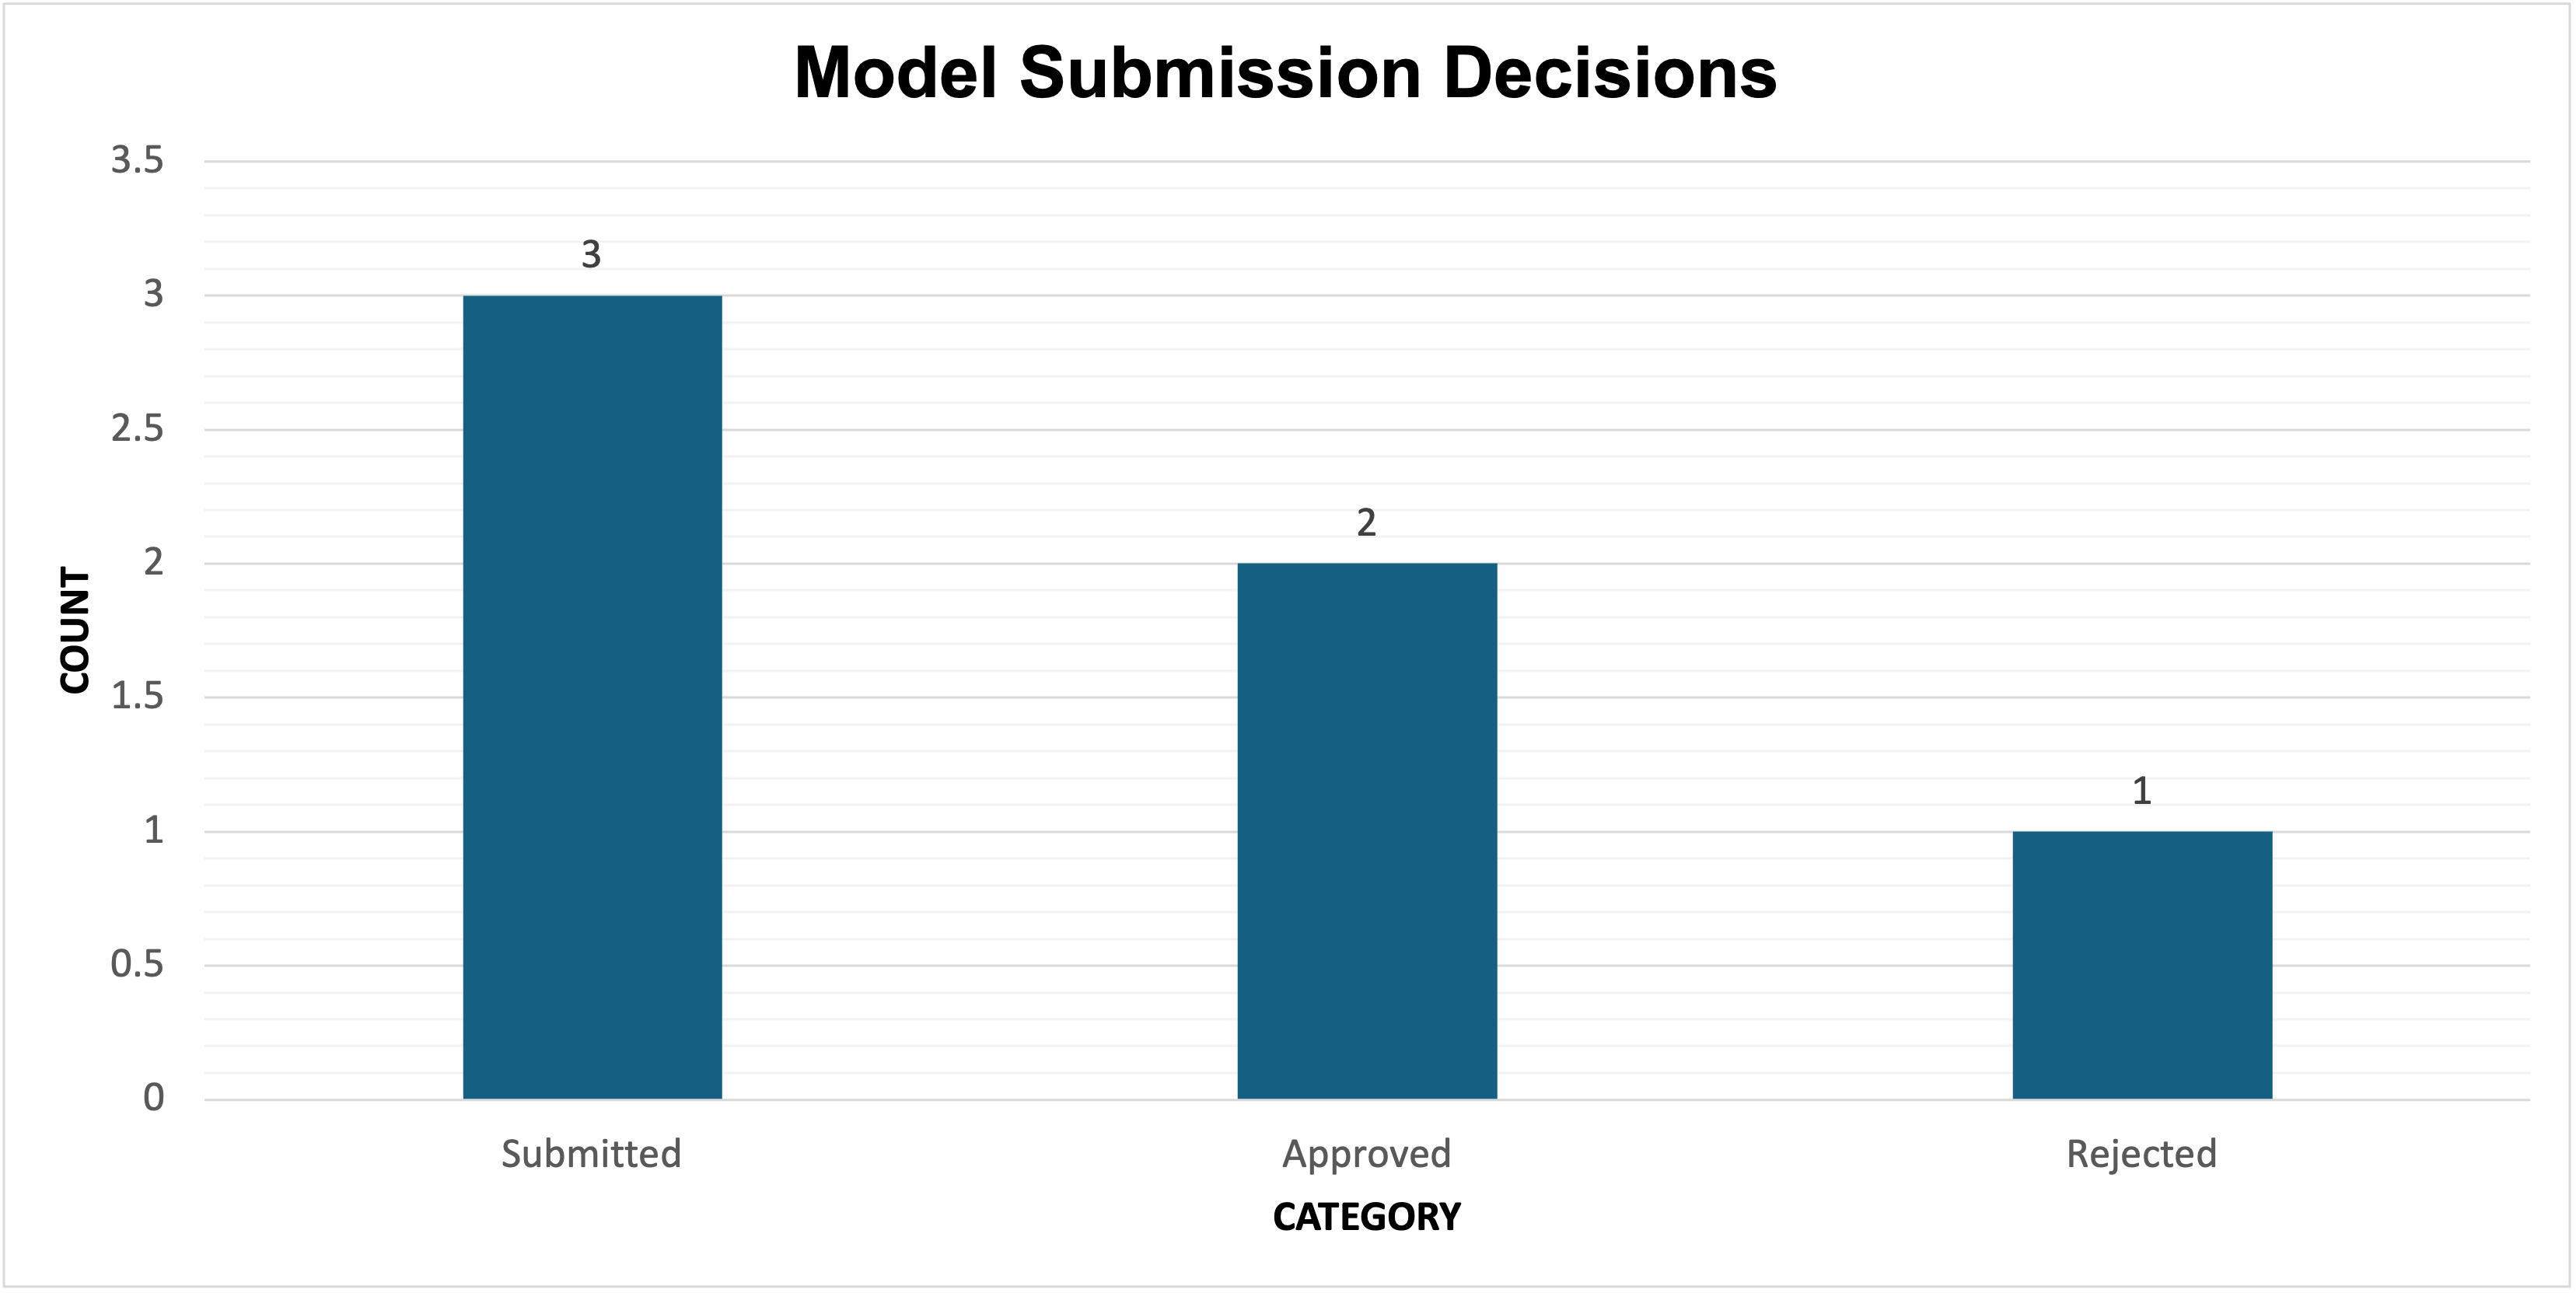
\includegraphics[width=\linewidth]{Figures/Results/fig1}
		
		\textbf{(a)} Submission Decisions
	\end{minipage}
	\hfill
	\begin{minipage}[t]{0.32\textwidth}
		\centering
		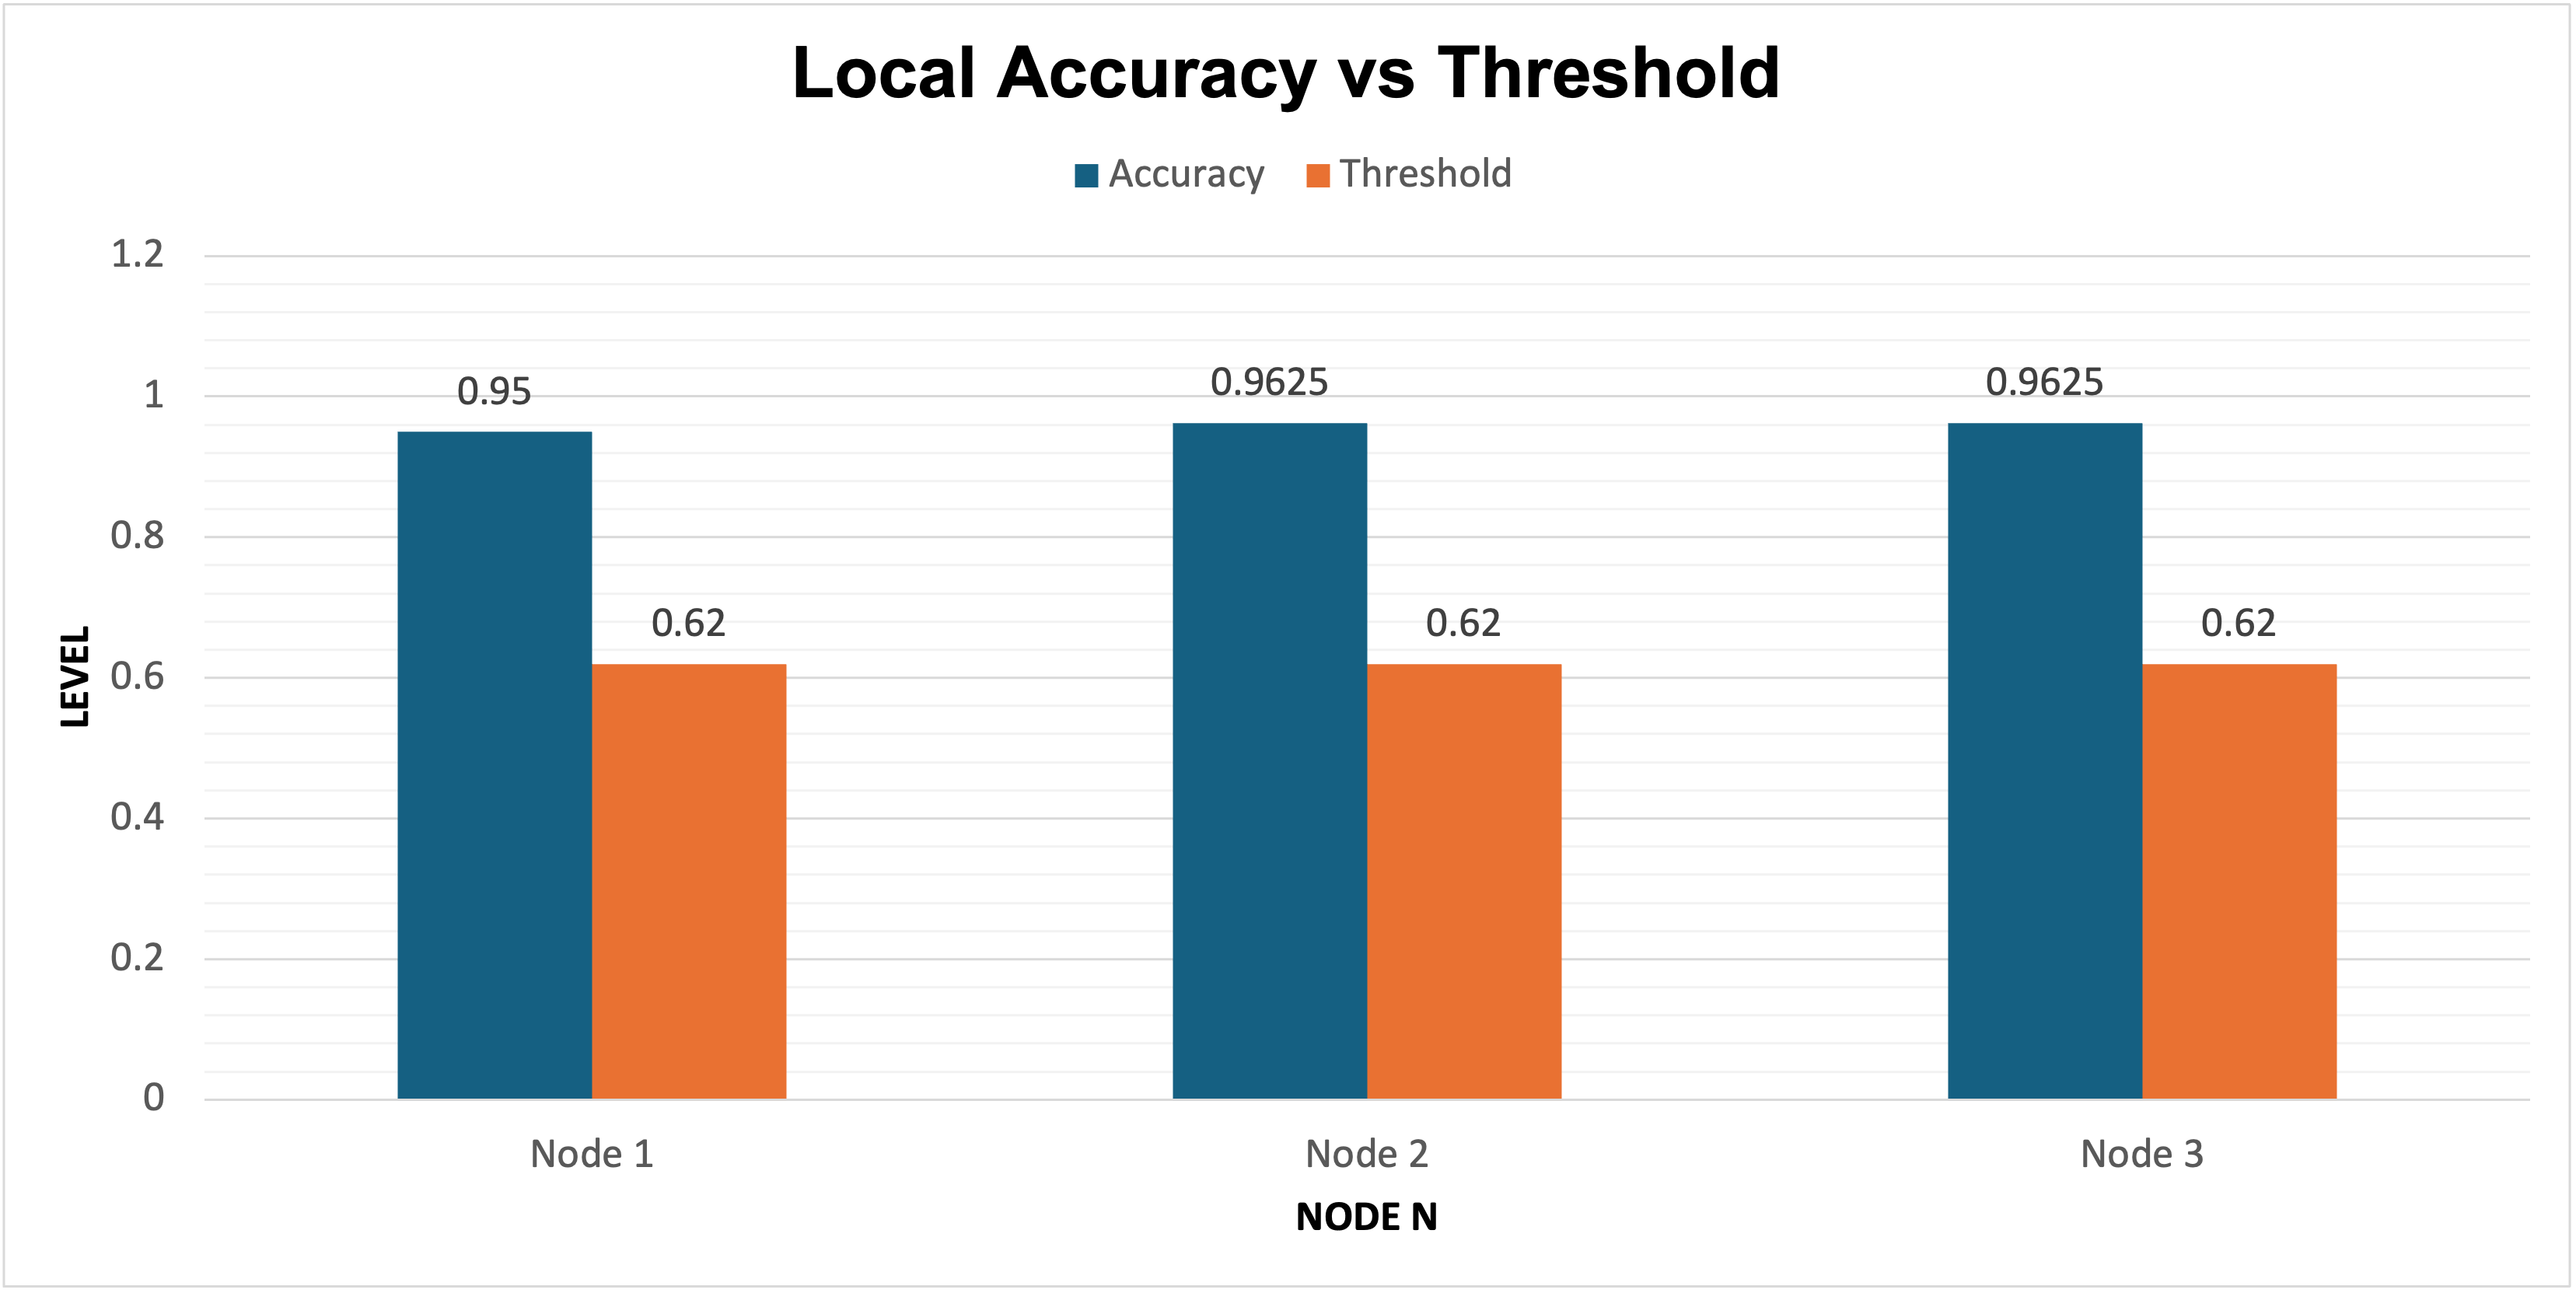
\includegraphics[width=\linewidth]{Figures/Results/fig2}
		
		\textbf{(b)} Accuracy Threshold
	\end{minipage}
	\hfill
	\begin{minipage}[t]{0.32\textwidth}
		\centering
		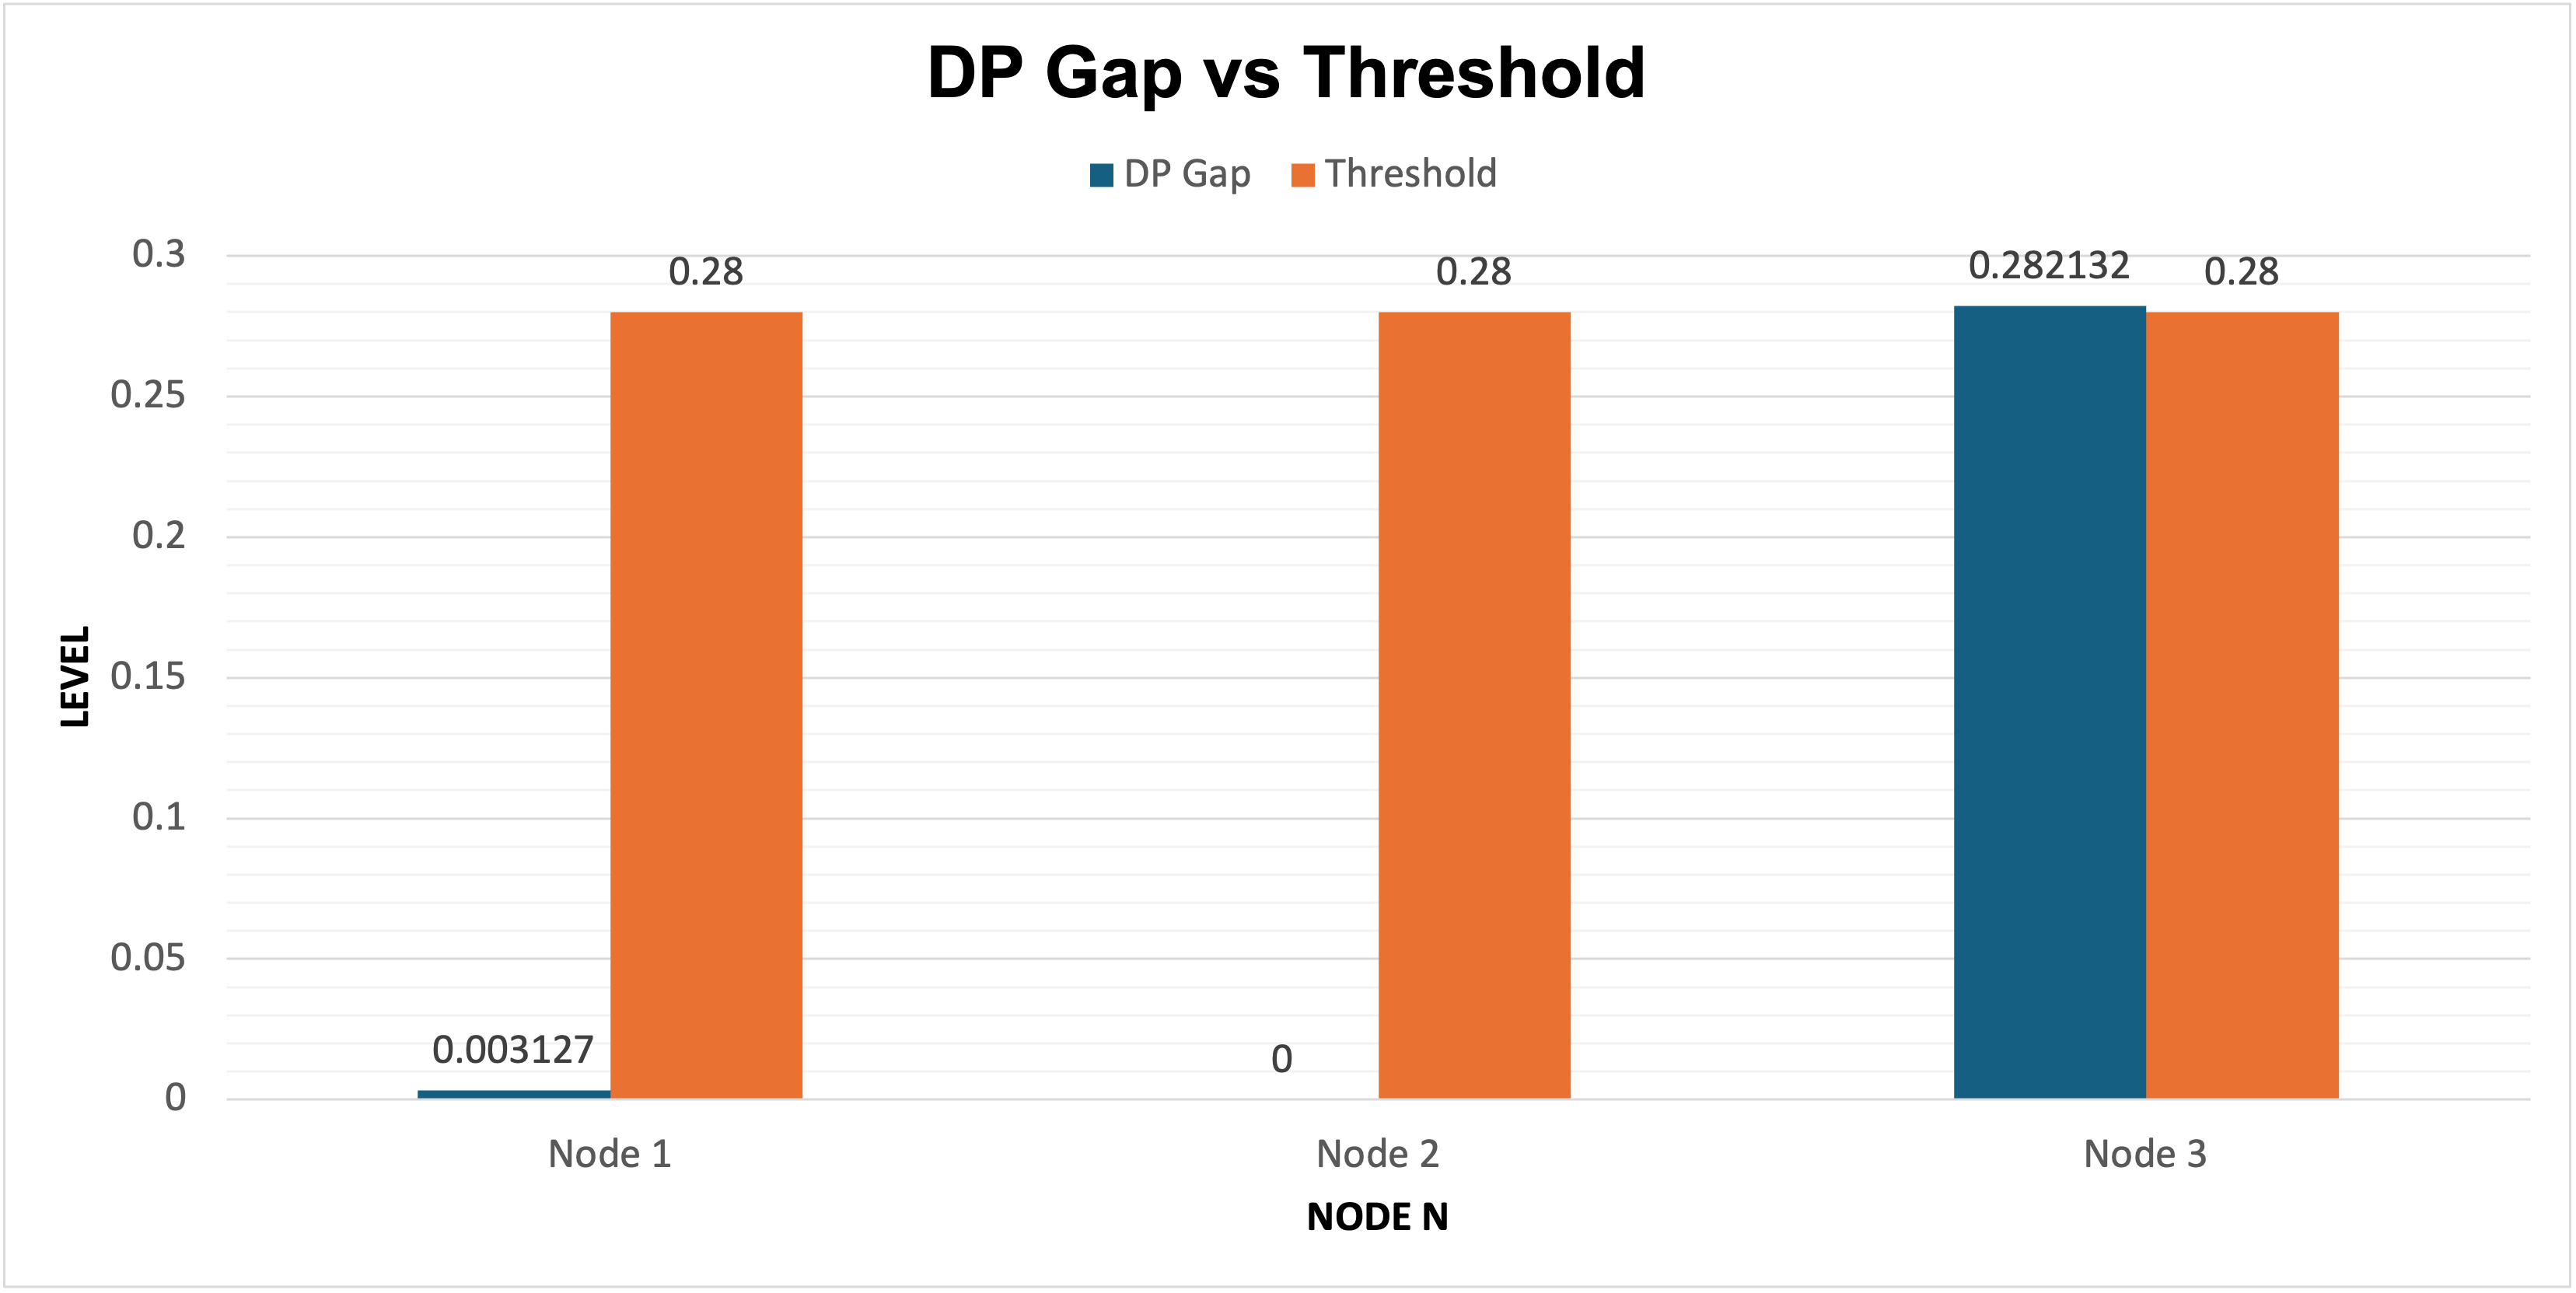
\includegraphics[width=\linewidth]{Figures/Results/fig3}
		
		\textbf{(c)} DP-Gap Threshold
	\end{minipage}
	
	\caption{Ethical Approval and Policy Compliance Results.}
	\label{fig:results-policy-compliance}
\end{figure*}

% ------------------------------------------------------------
\subsection{Proof-Based Verification and IPFS Traceability}
\label{subsec:results-proof-ipfs}
% ------------------------------------------------------------

Each local node generated a Groth16 proof using the \texttt{FairnessEligibility.circom} circuit. The proof checks policy compliance over public scaled metrics, including accuracy, demographic parity gap, policy thresholds, node identifier, and round identifier. Proofs were verified locally using \texttt{snarkjs}. The final on-chain decision was recorded through a signed verifier-service path: the verifier checked the Groth16 proof off-chain, signed the decision, \texttt{FairAISignedVerifier} verified the authorized signature on-chain, and \texttt{FairAIEthicalLedger} recorded the approval or rejection.

The node-level proof-generation times recorded in the final validation run were 846.173 ms for Node~1, 804.006 ms for Node~2, and 332.103 ms for Node~3. Across the three repeated trials, the trial-level mean proof-generation time was 629.425333 ms. Therefore, the node-level values and the repeated-trial mean describe different aggregation levels of the measurement. Figure~\ref{fig:results-proof-ipfs}(a) shows the node-level proof-generation times. The final result path did not use direct Solidity Groth16 verification; instead, it used signed on-chain decision recording after local Groth16 verification.

The final framework run used strict Kubo/IPFS storage. Each local node published model-related artifacts to IPFS, including model files, metrics, metadata, proof artifacts, public inputs, and manifests. The global model and evaluation summary were also published as IPFS artifacts. The result package records 20 tracked artifacts with CIDs, artifact types, storage mode, schema validation status, retrieval status, pin status, and artifact sizes where available. Figure~\ref{fig:results-proof-ipfs}(b) shows the artifact distribution by type, and Figure~\ref{fig:results-proof-ipfs}(c) reports the node-level artifact sizes. The strict \texttt{kubo-http} mode confirms that the storage path used the real Dockerized Kubo/IPFS service rather than a local hash-only fallback, and the exported validation records show that key retrieval and pin checks passed.

\begin{figure*}[htpb]
	\centering
	
	\begin{minipage}[t]{0.32\textwidth}
		\centering
		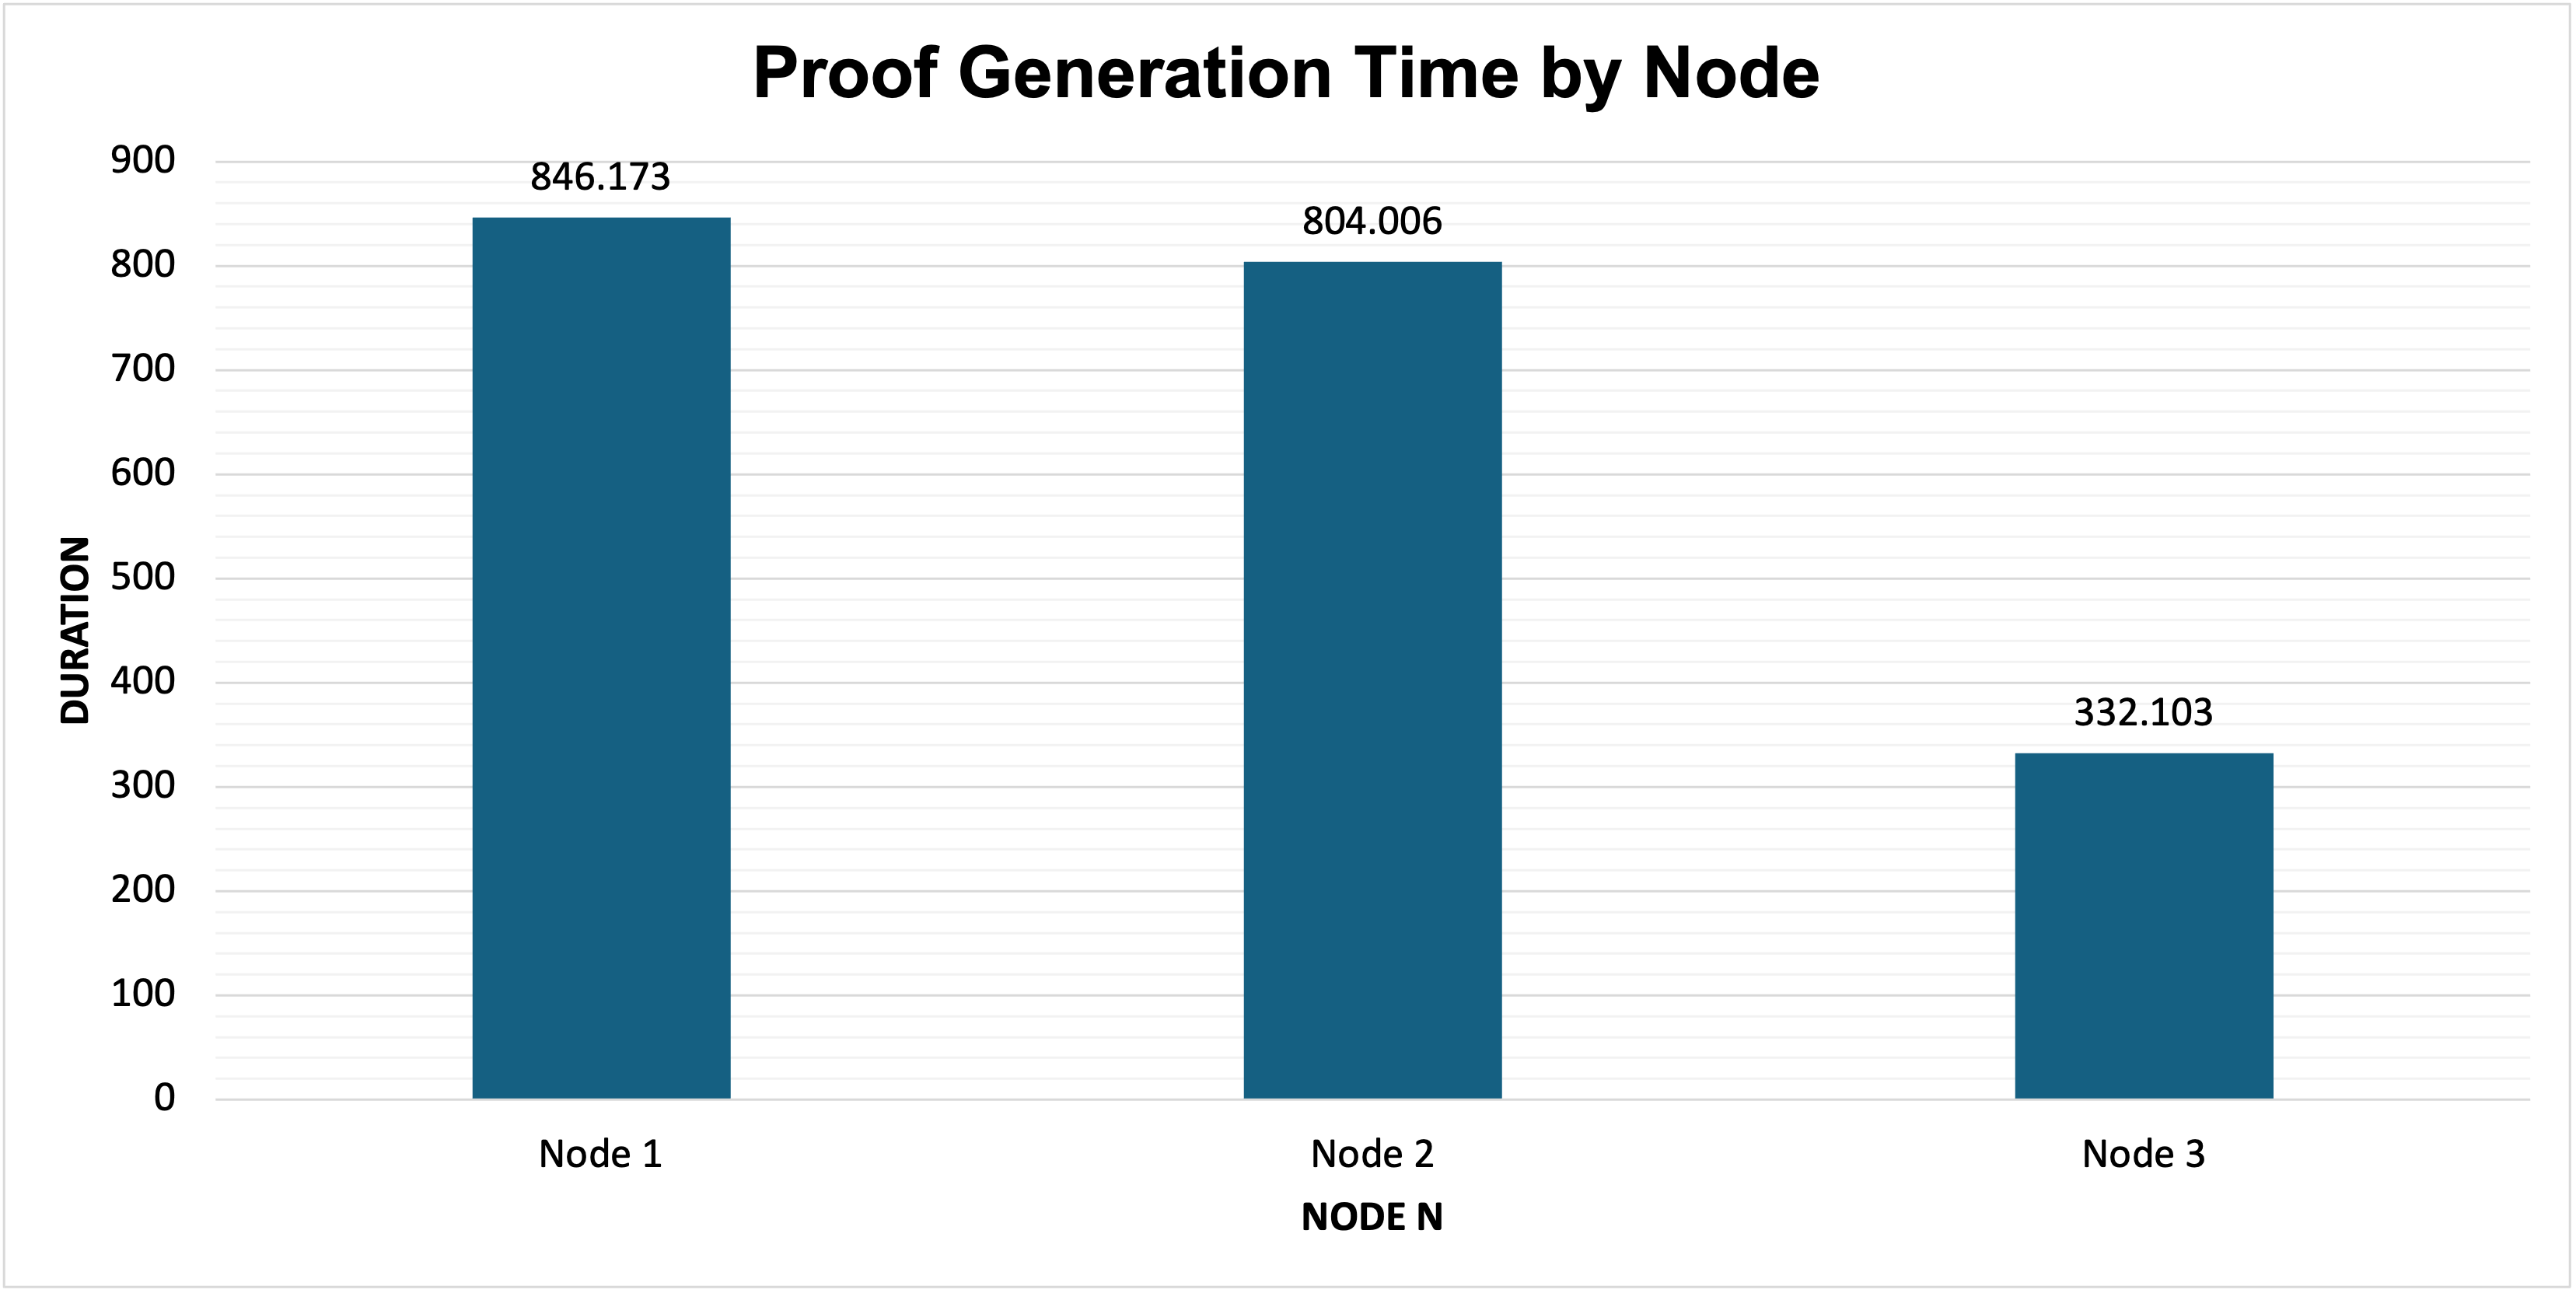
\includegraphics[width=\linewidth]{Figures/Results/fig4}
		
		\textbf{(a)} Proof Generation Time
	\end{minipage}
	\hfill
	\begin{minipage}[t]{0.32\textwidth}
		\centering
		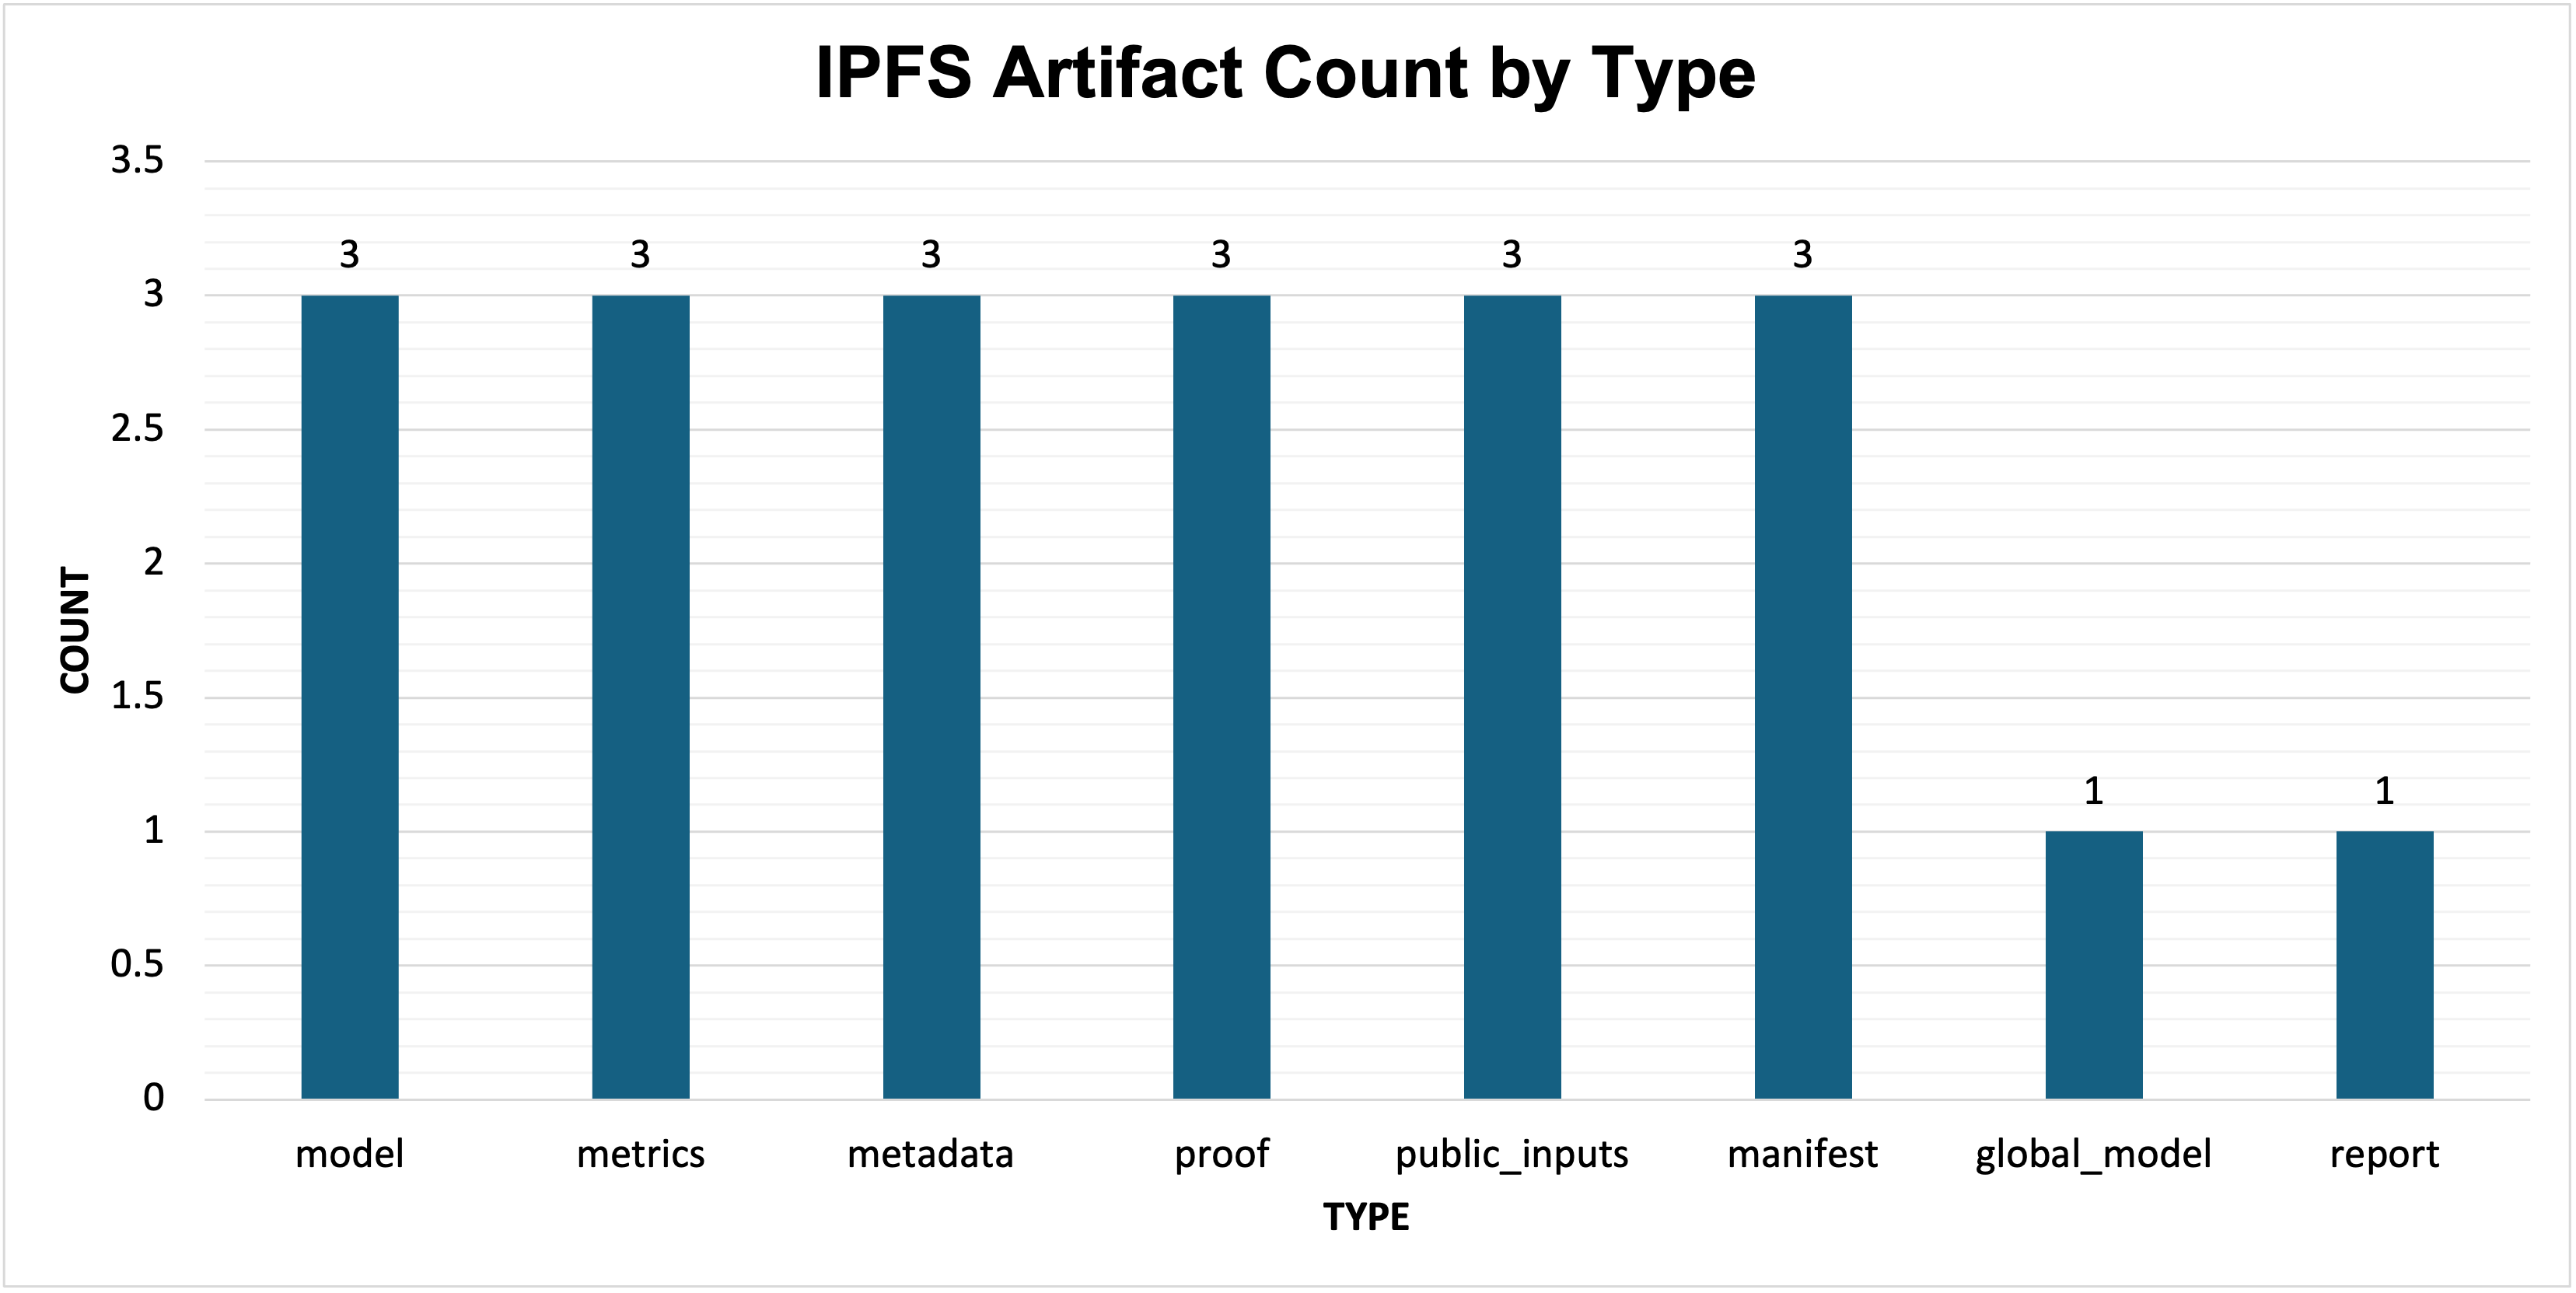
\includegraphics[width=\linewidth]{Figures/Results/fig5}
		
		\textbf{(b)} IPFS Artifact Count
	\end{minipage}
	\hfill
	\begin{minipage}[t]{0.32\textwidth}
		\centering
		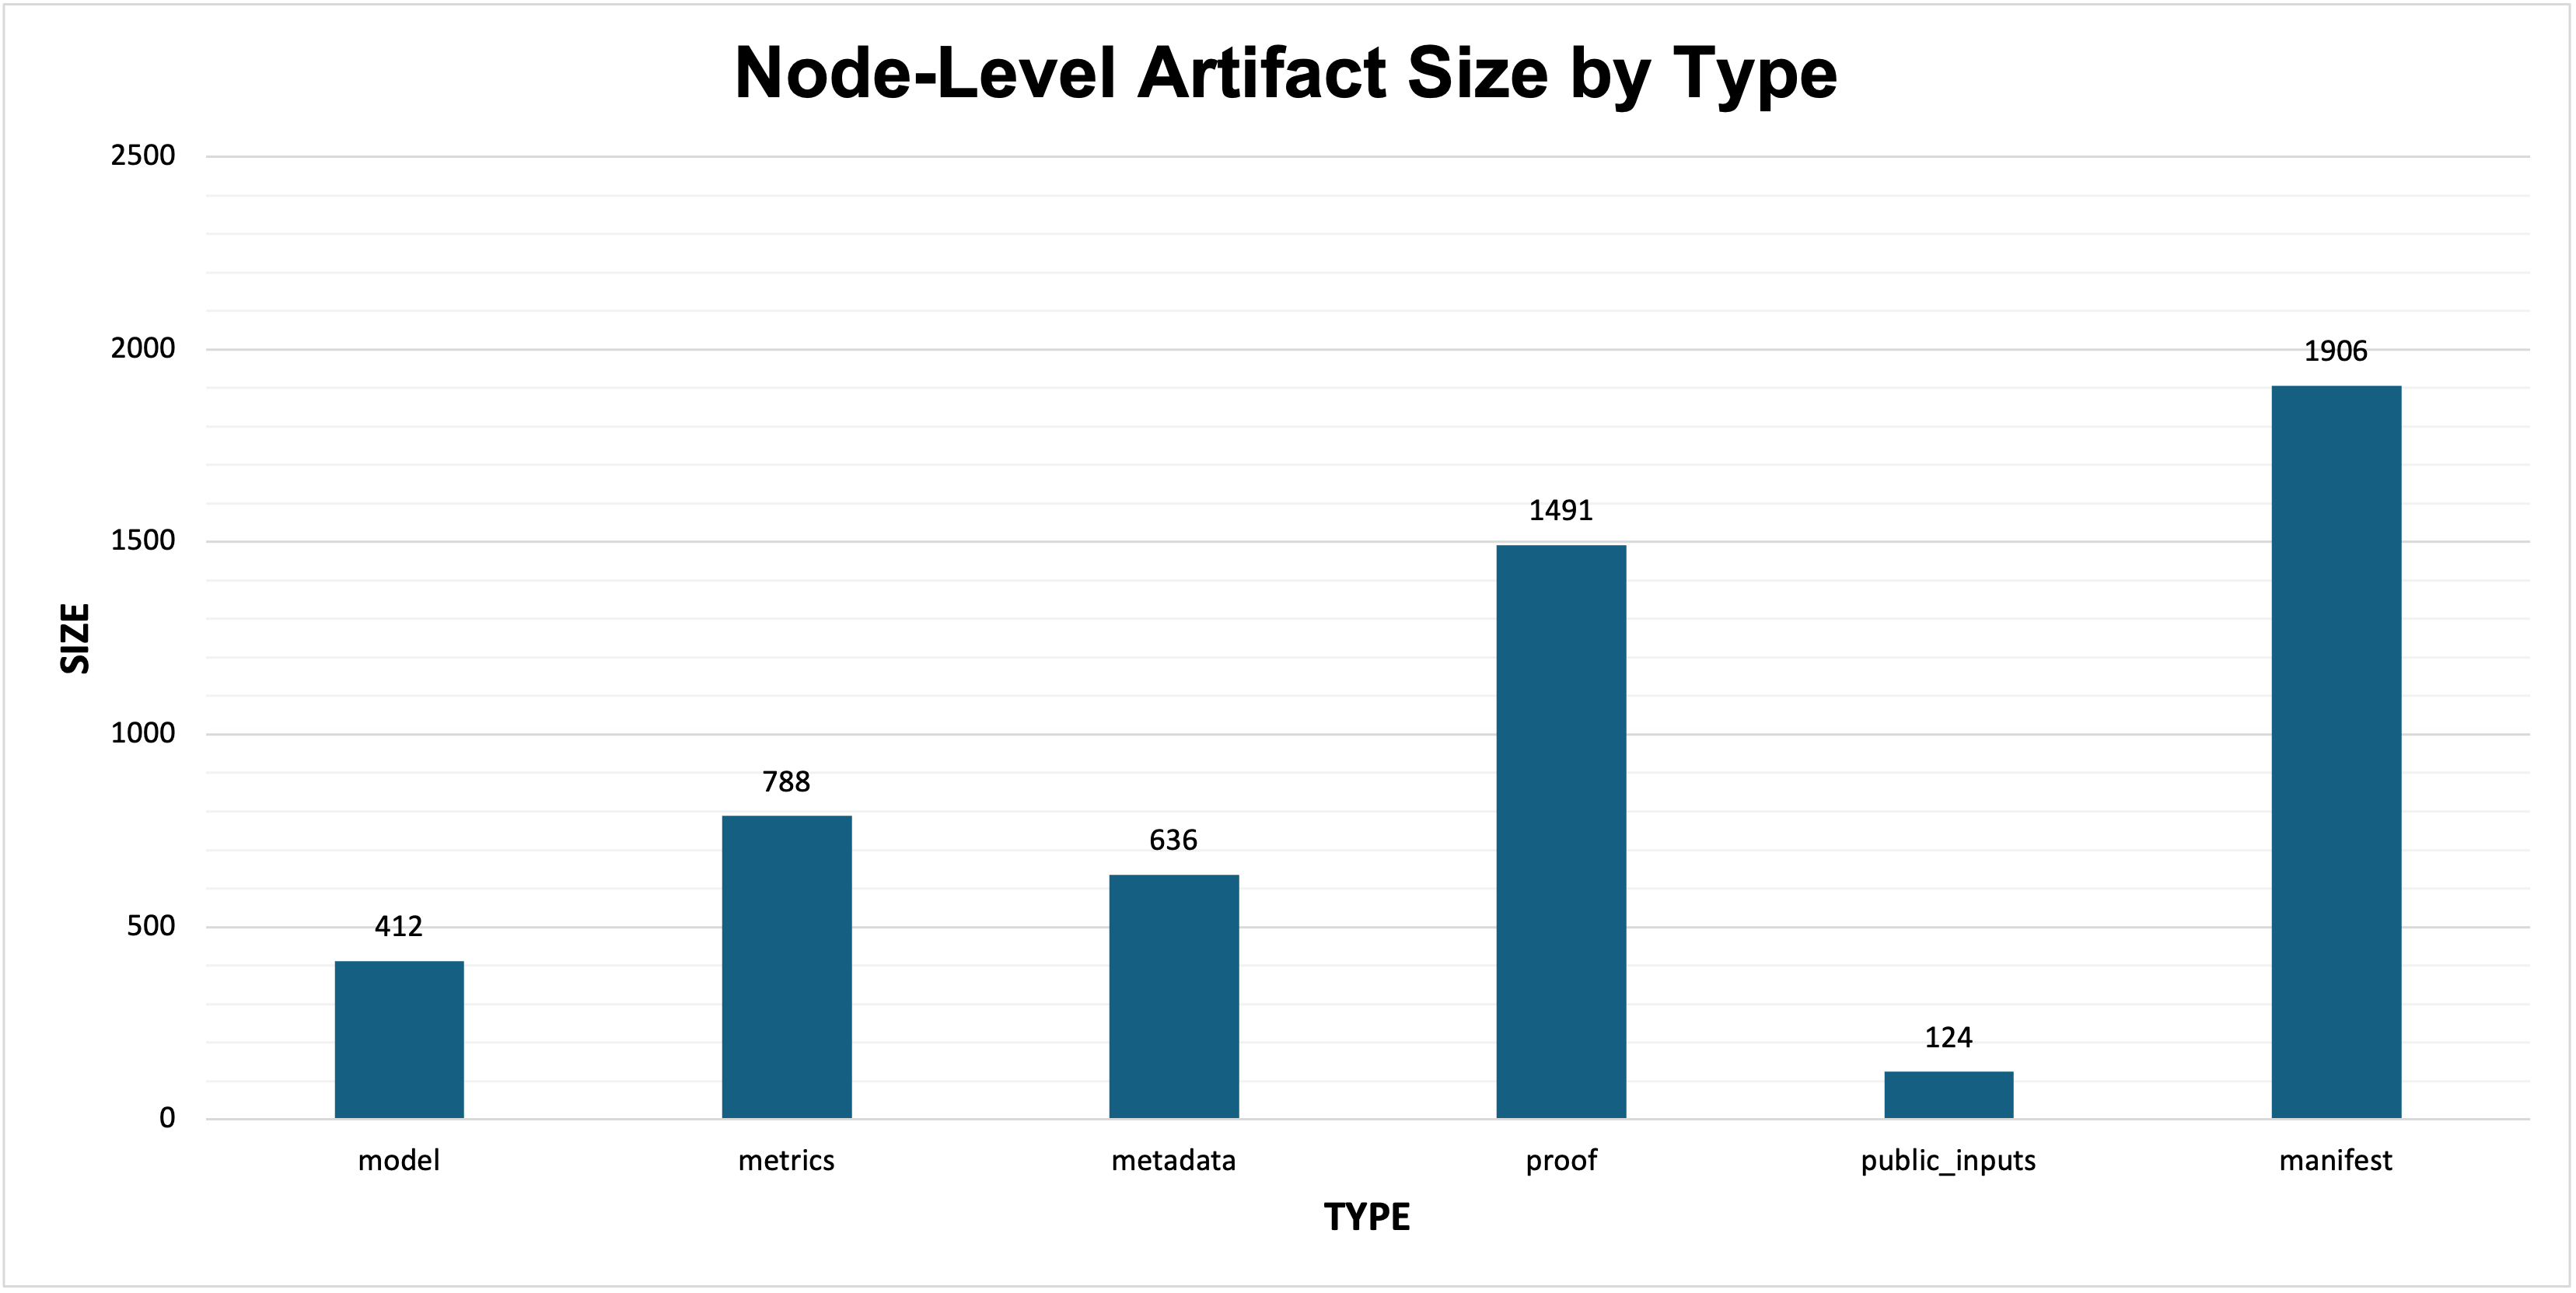
\includegraphics[width=\linewidth]{Figures/Results/fig6}
		
		\textbf{(c)} Artifact Size
	\end{minipage}
	
	\caption{Proof-Based Verification and IPFS Traceability Results.}
	\label{fig:results-proof-ipfs}
\end{figure*}

% ------------------------------------------------------------
\subsection{Approved-Only Aggregation and Global Publication}
\label{subsec:results-approved-aggregation}
% ------------------------------------------------------------

After verification, only approved local model artifacts were retrieved and aggregated. Node~1 and Node~2 formed the approved set, while Node~3 was excluded. The global model was computed using weighted FedAvg, with local sample count as the weighting factor. The resulting global model achieved a validation accuracy of \(0.938889\) and a demographic parity gap of \(0.144269\). Table~\ref{tab:results-global-publication} summarizes the approved-only aggregation and global publication results.

\begin{table}[htpb]
	\caption{Approved-Only Aggregation and Global Artifact Publication Results.}
	\label{tab:results-global-publication}
	\centering
	\scriptsize
	\renewcommand{\arraystretch}{1.08}
	\begin{tabular}{ll}
		\toprule
		\textbf{Metric} & \textbf{Value} \\
		\midrule
		Approved participants & \texttt{[1, 2]} \\
		Rejected participants & \texttt{[3]} \\
		Aggregation method & Weighted FedAvg \\
		Weighting factor & Local sample count \\
		Global validation accuracy & 0.938889 \\
		Global demographic parity gap & 0.144269 \\
		Global model CID & \texttt{bafkreihanoztcqq4p...aupccjn4zm} \\
		Evaluation summary CID & \texttt{bafkreigkcm7b4wwix...rae3nqljem} \\
		Global publication gas & 449664 \\
		\bottomrule
	\end{tabular}
\end{table}

The result demonstrates that FairAI can produce a global model while excluding a non-compliant participant from the aggregation set. The global model and evaluation summary were published as content-addressed artifacts, preserving traceability between approved inputs and final outputs.

% ------------------------------------------------------------
\subsection{Audit, Gas, and Repeated-Trial Measurements}
\label{subsec:results-audit-repeated}
% ------------------------------------------------------------

The contract logs recorded gas usage for node submission/audit events and global publication. Node~1 submission/audit logging used 760819 gas, Node~2 used 743695 gas, Node~3 used 717757 gas, and global publication used 449664 gas. Table~\ref{tab:results-gas} reports the captured gas usage, and Figure~\ref{fig:results-cost-performance}(a) visualizes the same measurements.

\begin{table}[htpb]
	\caption{Captured Gas Usage for Submission/Audit Events and Global Publication.}
	\label{tab:results-gas}
	\centering
	\scriptsize
	\renewcommand{\arraystretch}{1.08}
	\begin{tabular}{lcc}
		\toprule
		\textbf{Event} & \textbf{Node / Scope} & \textbf{Gas Used} \\
		\midrule
		Model submission and audit & Node 1 & 760819 \\
		Model submission and audit & Node 2 & 743695 \\
		Model submission and audit & Node 3 & 717757 \\
		Global model publication & Global & 449664 \\
		\bottomrule
	\end{tabular}
\end{table}

The final experiment runner executed three repeated trials. The mean approval rate was \(0.666667\), the mean global accuracy was \(0.938889\), and the mean global demographic parity gap was \(0.144269\). The mean proof-generation time was 629.425333 ms, the mean IPFS retrieval time was 0.928381 ms, and the mean runtime was 3165.868667 ms. Table~\ref{tab:results-repeated-trials} summarizes the repeated-trial framework metrics. Figure~\ref{fig:results-cost-performance}(b) visualizes the aggregate approval, performance, and fairness metrics, while Figure~\ref{fig:results-cost-performance}(c) visualizes the main overhead metrics.

\begin{table}[htpb]
	\caption{Repeated-Trial Framework Metrics.}
	\label{tab:results-repeated-trials}
	\centering
	\scriptsize
	\renewcommand{\arraystretch}{1.08}
	\begin{tabular}{lcc}
		\toprule
		\textbf{Metric} & \textbf{Mean / Value} & \textbf{Std.} \\
		\midrule
		Trials & 3.000000 & 0.000000 \\
		Approval rate & 0.666667 & 0.000000 \\
		Global accuracy & 0.938889 & 0.000000 \\
		Global demographic parity gap & 0.144269 & 0.000000 \\
		Proof generation time (ms) & 629.425333 & 4.905826 \\
		IPFS retrieval time (ms) & 0.928381 & 0.060721 \\
		Runtime (ms) & 3165.868667 & 9.652791 \\
		Global publication gas & 449664.000000 & 0.000000 \\
		\bottomrule
	\end{tabular}
\end{table}

The repeated trials show stable framework behavior under the tested configuration. The same approval pattern was preserved across trials, and the measured proof, retrieval, and runtime values showed low variation. These values quantify the cost of the smart-contract governance path and show that approvals, rejections, and global publication are recorded as auditable blockchain events.

\begin{figure*}[htpb]
	\centering
	
	\begin{minipage}[t]{0.32\textwidth}
		\centering
		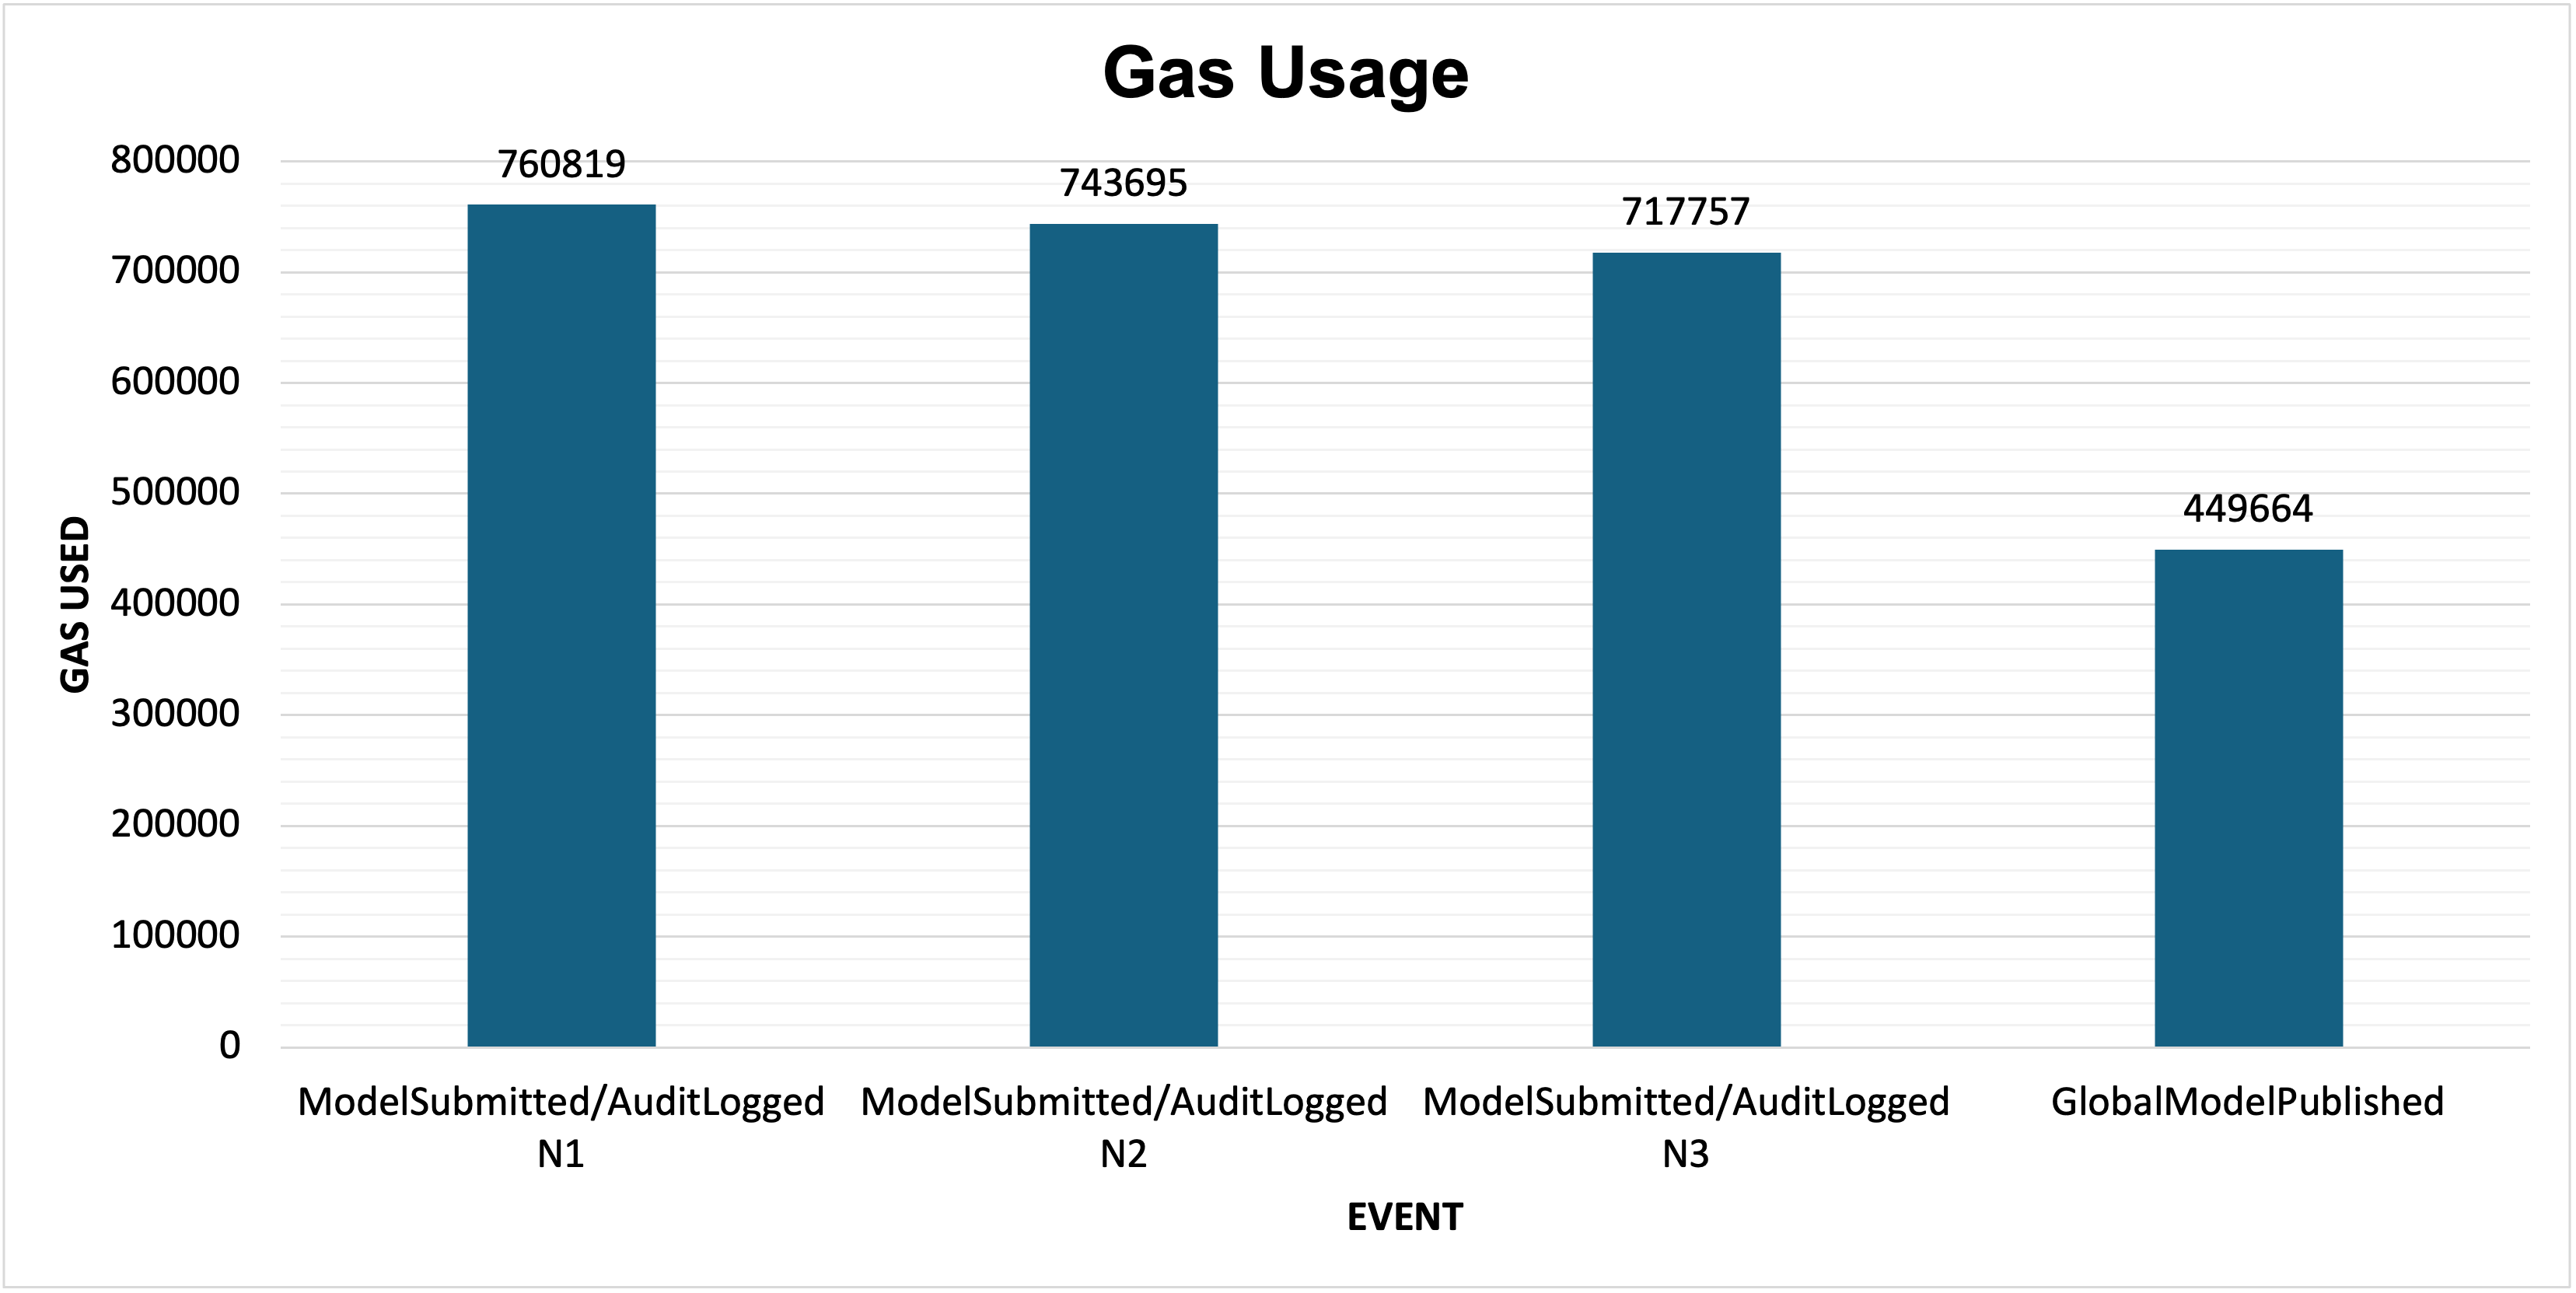
\includegraphics[width=\linewidth]{Figures/Results/fig9}
		
		\textbf{(a)} Gas Usage
	\end{minipage}
	\hfill
	\begin{minipage}[t]{0.32\textwidth}
		\centering
		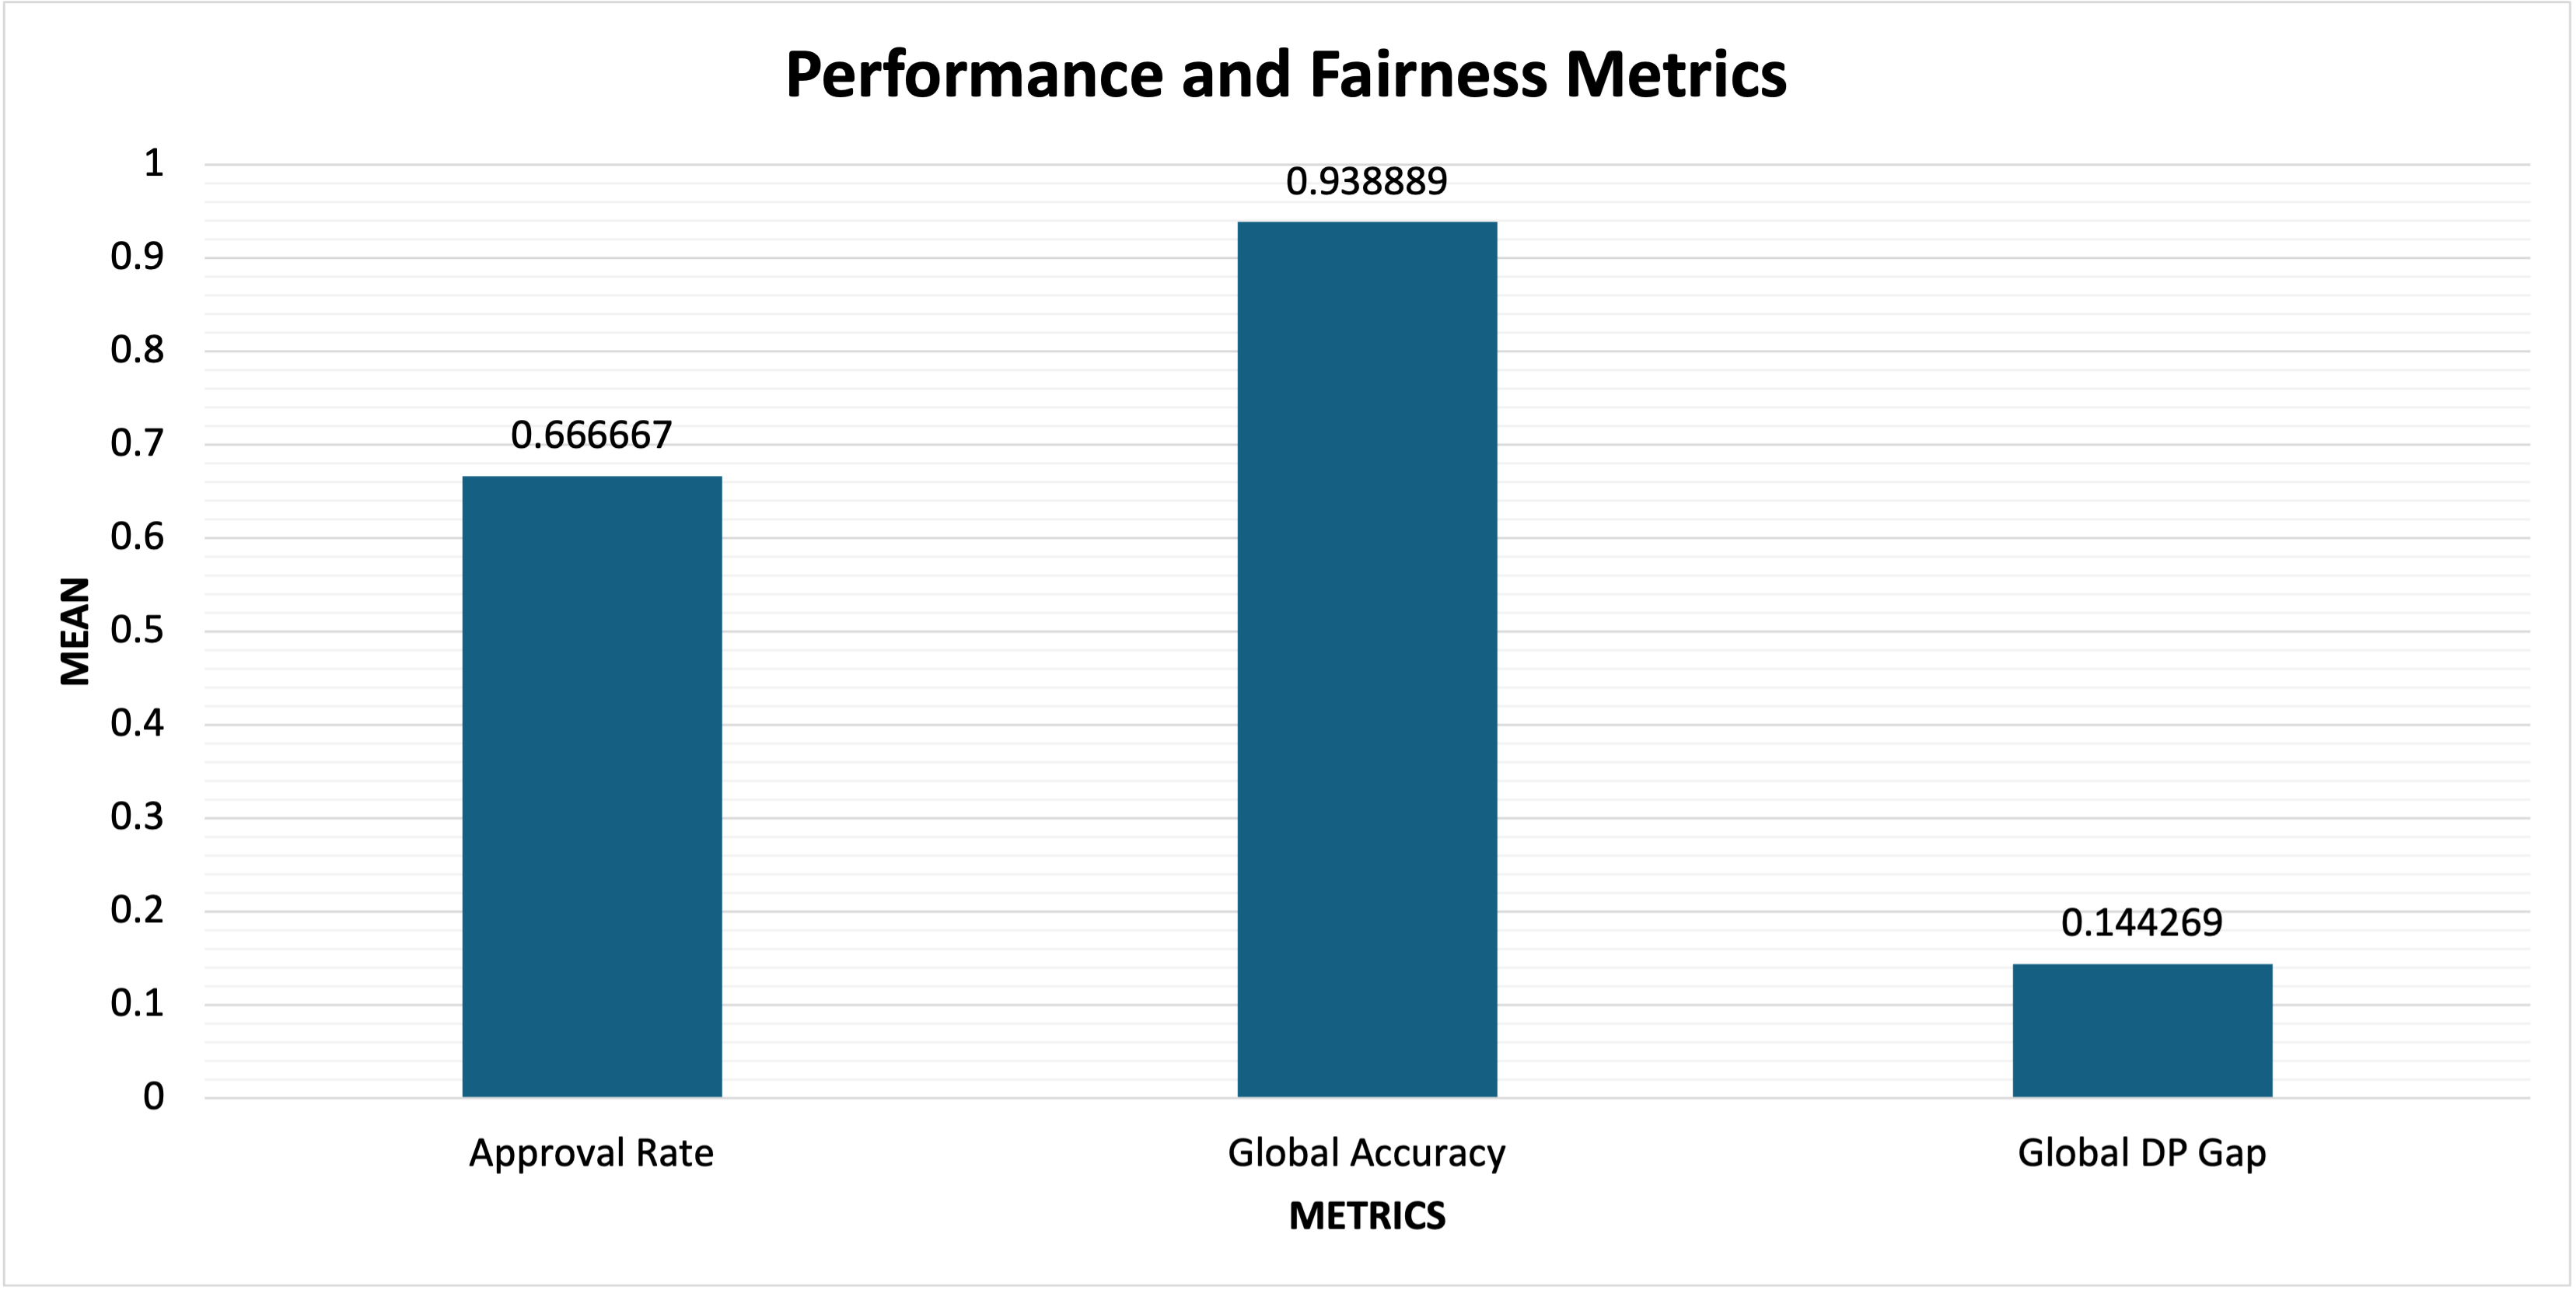
\includegraphics[width=\linewidth]{Figures/Results/fig8}
		
		\textbf{(b)} Performance and Fairness
	\end{minipage}
	\hfill
	\begin{minipage}[t]{0.32\textwidth}
		\centering
		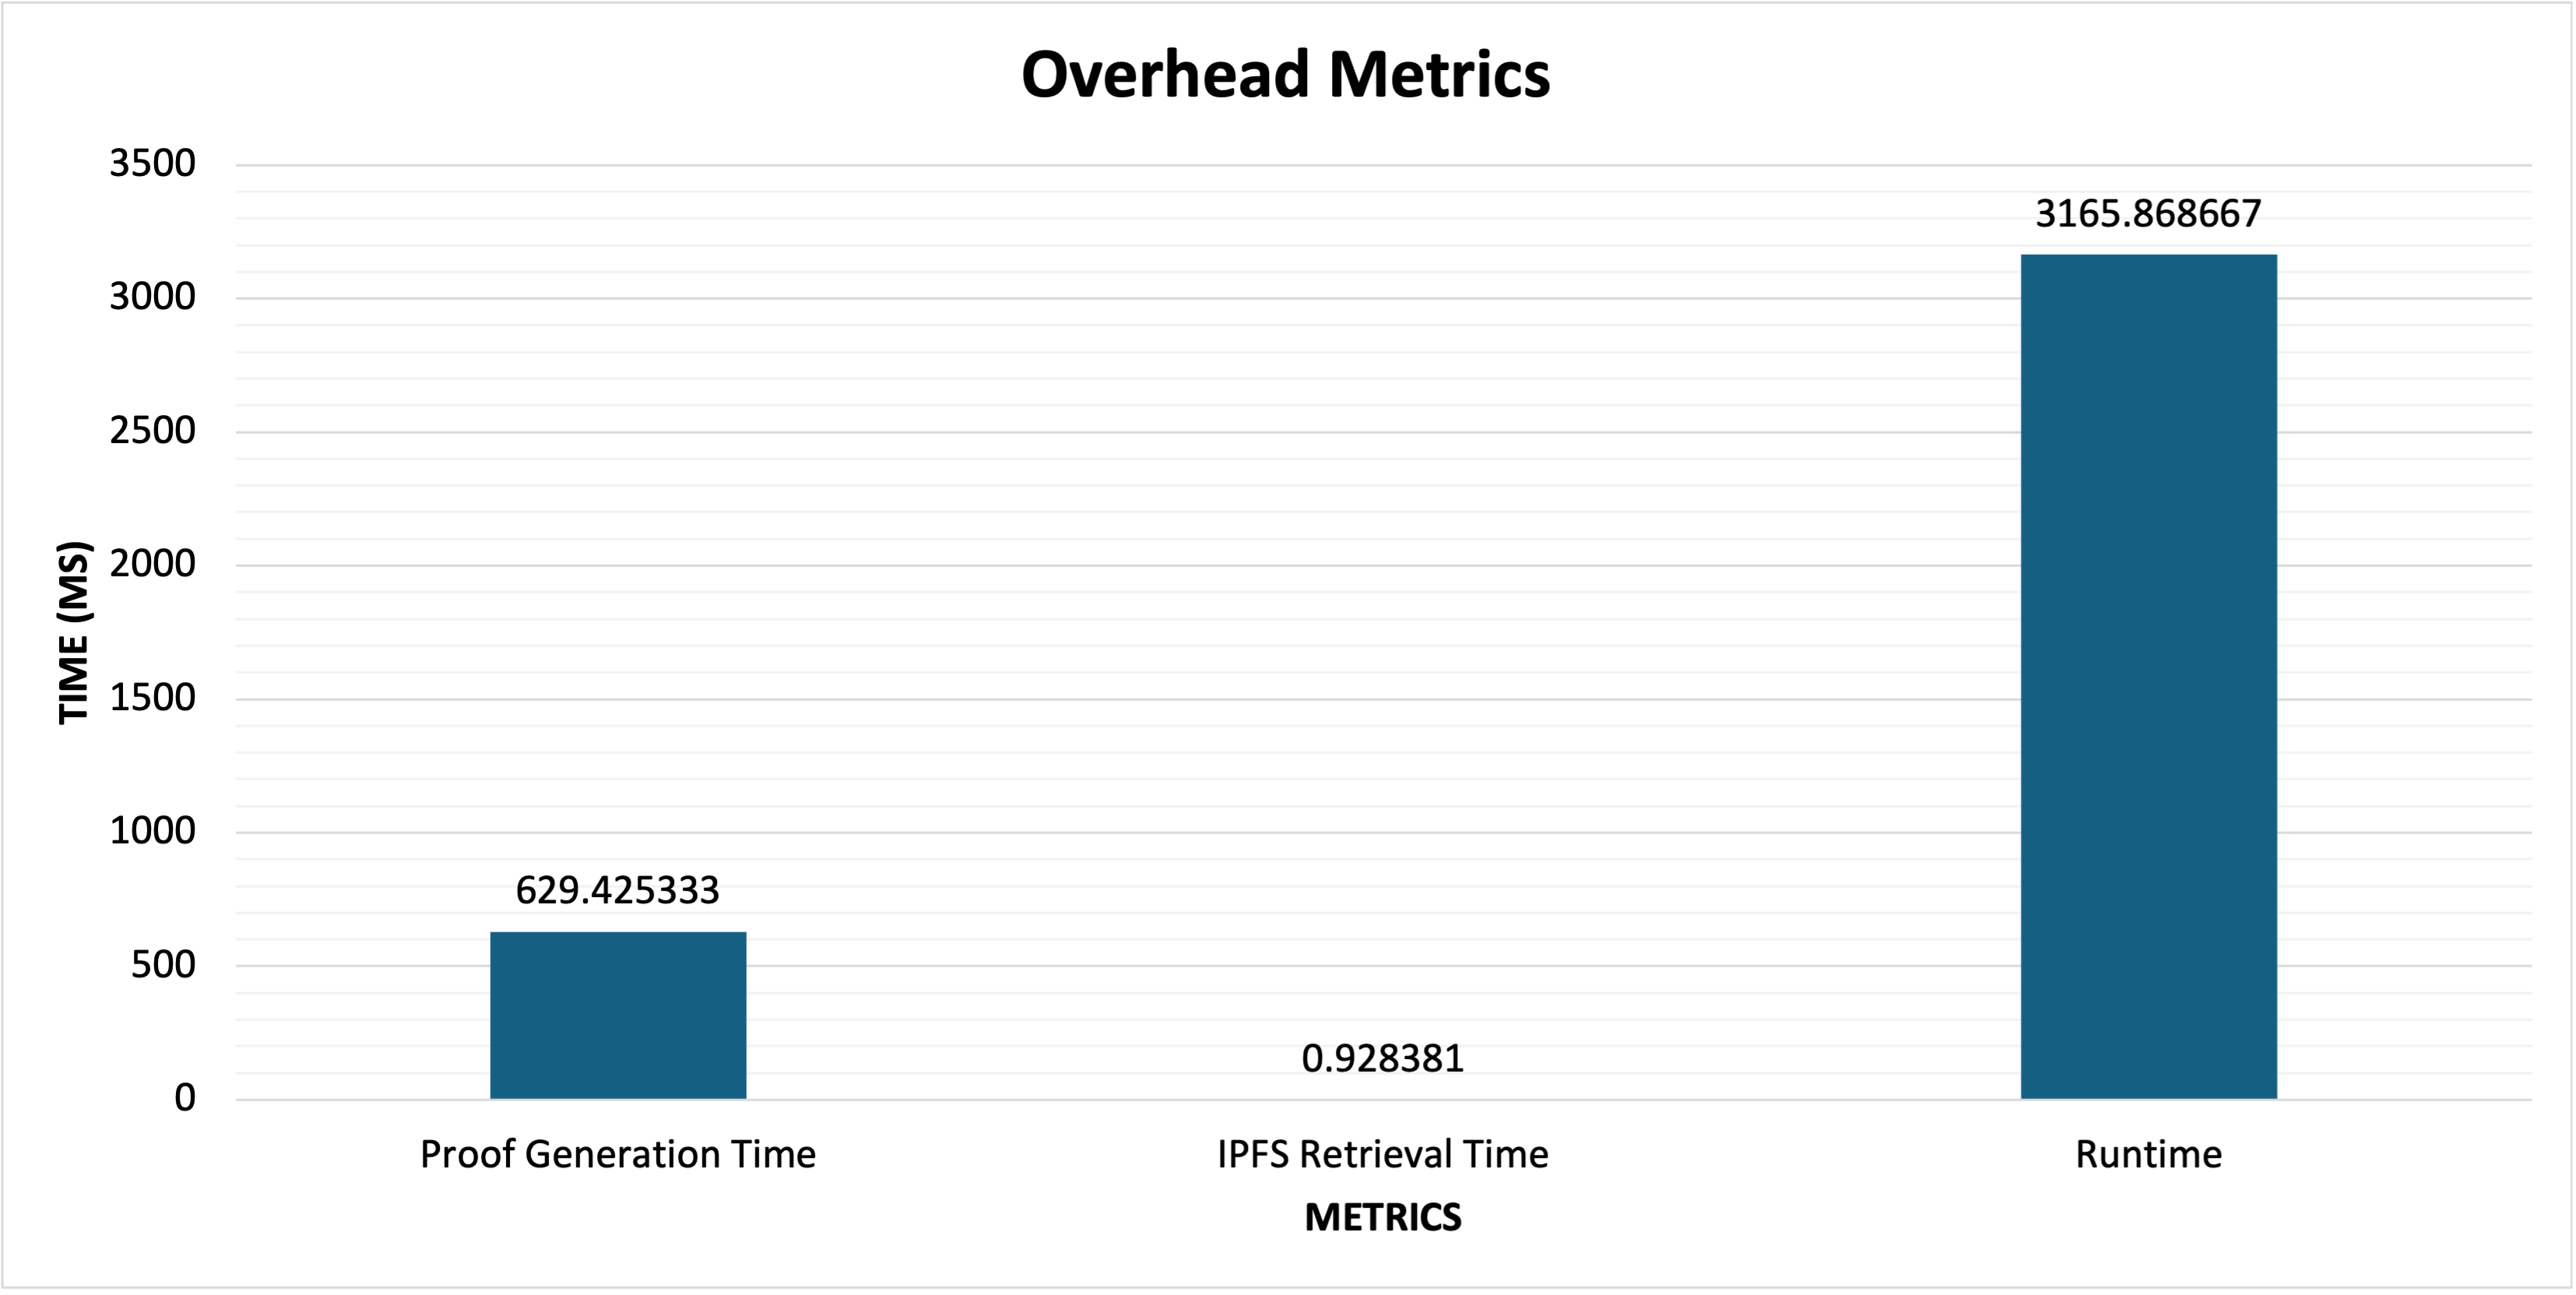
\includegraphics[width=\linewidth]{Figures/Results/fig7}
		
		\textbf{(c)} Overhead Metrics
	\end{minipage}
	
	\caption{Governance Cost and Repeated-Trial Results.}
	\label{fig:results-cost-performance}
\end{figure*}

% ------------------------------------------------------------
\subsection{Framework Validation Summary}
\label{subsec:results-validation-summary}
% ------------------------------------------------------------

Table~\ref{tab:results-validation-checklist} summarizes the validated FairAI properties. The results confirm that the framework can preserve local data privacy, publish artifacts to IPFS, register CIDs and verification states through smart contracts, execute Groth16 proof generation and local verification, record signed verifier decisions, reject non-compliant models, aggregate only approved local models, publish the global model, and archive the round.

\begin{table}[htpb]
	\caption{FairAI Framework Validation Checklist.}
	\label{tab:results-validation-checklist}
	\centering
	\scriptsize
	\renewcommand{\arraystretch}{1.08}
	\begin{tabular}{lc}
		\toprule
		\textbf{Framework property} & \textbf{Validated} \\
		\midrule
		Raw local training data remain off-chain & Yes \\
		Strict Kubo/IPFS artifact storage used & Yes \\
		Model, metrics, proof, public-input, metadata, and manifest artifacts stored & Yes \\
		CIDs and verification states recorded through governance path & Yes \\
		Groth16 proof generation executed & Yes \\
		Local \texttt{snarkjs} proof verification executed & Yes \\
		Signed verifier-service on-chain decision path executed & Yes \\
		Smart-contract approval/rejection recorded & Yes \\
		Fairness-noncompliant node rejected & Yes \\
		Only approved nodes aggregated & Yes \\
		Global model and evaluation summary published as CIDs & Yes \\
		Round archived & Yes \\
		\bottomrule
	\end{tabular}
\end{table}

The framework validation confirms that FairAI implements ethical FL as a governed artifact workflow. The system does not simply train and aggregate local models; it records which artifacts were submitted, how they were verified, which models were approved or rejected, and which approved artifacts shaped the final global output.
% ============================================================
% ============================================================
\section{Discussion}
\label{sec:discussion}
% ============================================================

The final FairAI validation demonstrates that ethical federated learning can be operationalized as a governed model-artifact workflow rather than as a post-hoc evaluation step. The results show that local models can be trained privately, packaged as traceable artifacts, verified against an eligibility policy, recorded through smart-contract governance, and selectively aggregated only when approved. This directly supports the approval-gated model formalized in Eq. \eqref{eq:approval-gate-model} and the approved-only aggregation rule in Eq. \eqref{eq:approved-fedavg}. In contrast to conventional FL, where participation often determines whether an update enters the aggregation pool, FairAI makes aggregation eligibility an auditable governance decision.

The results provide evidence for three main framework-level claims. First, FairAI enforces ethical eligibility before aggregation. Table \ref{tab:results-node-eligibility} and Figure \ref{fig:results-policy-compliance} show that Node~1 and Node~2 satisfied the configured accuracy and demographic parity constraints, while Node~3 was rejected because its demographic parity gap exceeded the configured threshold. This is important because the rejected node still achieved high local accuracy, demonstrating that accuracy alone is insufficient for ethical aggregation. This finding is consistent with fairness-aware FL research showing that fairness, privacy, heterogeneity, and aggregation behavior can interact in complex ways \cite{intro_4,intro_5,rw_16}. FairAI does not assume that one fairness metric is universally sufficient; rather, it provides a mechanism for enforcing configurable ethical policies before the global model is updated.

Second, FairAI provides traceable and auditable model provenance. The IPFS-backed artifact model stores local models, proof artifacts, metrics, metadata, public inputs, and manifests off-chain, while CIDs and verification decisions are recorded through the governance path. Figure \ref{fig:results-proof-ipfs} summarizes the proof-generation and IPFS artifact-traceability results, and Table \ref{tab:results-validation-checklist} confirms that the framework validated strict Kubo/IPFS storage, CID registration, proof generation, local verification, signed verifier-service decision recording, and lifecycle archival. This follows the blockchain--IPFS pattern in which large artifacts remain outside the ledger while immutable references are stored on-chain \cite{intro_8,rw_21}. In FairAI, however, CIDs are not only storage references; they connect each submitted model to its verification status, approval decision, and aggregation eligibility.

Third, FairAI remains operational after enforcing the approval gate. Table \ref{tab:results-global-publication} shows that only the two approved local models were aggregated, producing a global validation accuracy of \(0.938889\) and a demographic parity gap of \(0.144269\). These values should be interpreted as feasibility indicators rather than as the sole contribution of the work. The central contribution is that the final global model was built only from artifacts that passed the governance workflow. The repeated-trial results in Table \ref{tab:results-repeated-trials} and Figure \ref{fig:results-cost-performance} further show stable approval rate, global accuracy, fairness gap, proof-generation time, IPFS retrieval time, runtime, and global publication gas under the tested configuration.

The verification pathway also clarifies the role of proof-based governance in FairAI. In the reported implementation, Groth16 proofs are generated from the eligibility circuit and checked locally using \texttt{snarkjs}; the on-chain decision is then recorded through a signed verifier-service path. This architecture separates proof computation from governance recording: the verifier checks the proof and signs the decision, while the contract verifies the authorized decision and records the approval or rejection. This design is consistent with recent verifiable-FL work in which proof systems support privacy-preserving verification of distributed learning claims \cite{intro_9,intro_10,intro_14,rw_22}. It also keeps FairAI modular, since the same governance workflow can support direct on-chain verification, signed verifier services, or future optimized ZKP verification backends.

The measured overhead is expected because FairAI introduces governance stages that are absent from baseline FL: artifact publication, proof generation, CID registration, signed verification, contract logging, approved-only retrieval, and auditable global publication. The gas measurements in Table \ref{tab:results-gas} quantify the on-chain cost of recording node submissions/audit events and global publication. These costs are not incidental; they represent the cost of auditability, traceability, and enforceability. In production deployments, this trade-off can be tuned through batching, proof optimization, storage-gateway optimization, permissioned deployment, or alternative verification backends.

FairAI also complements robust FL defenses. Byzantine-resilient aggregation methods typically attempt to reduce the effect of malicious updates after they enter the candidate update pool \cite{intro_13,rw_26,rw_27,rw_28}. FairAI acts earlier: a local model must pass the approval workflow before it becomes eligible for retrieval and aggregation. This creates a pre-aggregation governance boundary that can prevent policy-violating, unverifiable, or unauthorized artifacts from influencing the global model. The framework also improves non-repudiation because submissions, CIDs, decisions, and publication records are logged through the governance layer.

The evaluation remains a framework validation. The workload uses three local nodes, synthetic local datasets, logistic regression, and three repeated trials. These choices are appropriate for validating the complete FairAI governance path, but larger deployments, additional datasets, more complex models, and broader adversarial settings are needed to characterize scalability and generalization. In addition, direct Solidity Groth16 verification remains a separate integration path, and richer fairness policies with domain-specific protected attributes should be evaluated in future work. Overall, the findings support the central claim of this paper: ethical FL can be implemented as an auditable approval-gated workflow over model artifacts, rather than as a post-hoc assessment of a completed global model.

% ------------------------------------------------------------
\subsection{Comparative Analysis}
\label{subsec:discussion-comparative-analysis}
% ------------------------------------------------------------

To contextualize the findings, Table \ref{tab:comparative-analysis-results} compares FairAI with recent research streams in trustworthy FL, fairness-aware FL, blockchain-based FL, IPFS-assisted decentralized storage, ZKP-based verifiable FL, and robust FL. Unlike prior approaches that typically focus on one or two trust dimensions, the final FairAI validation combines IPFS artifact storage, on-chain CID/status recording, Groth16 proof generation, signed verifier-service decisions, ethical rejection, approved-only aggregation, and global CID publication in one governance workflow.

\begin{table*}[htpb]
	\caption{Comparative Analysis. 
		\(\checkmark\): explicit support; \(\triangle\): partial support; --: not a primary focus.}
	\label{tab:comparative-analysis-results}
	\centering
	\scriptsize
	\setlength{\tabcolsep}{2.2pt}
	\renewcommand{\arraystretch}{1.05}
	
	\begin{tabularx}{\textwidth}{
			@{}
			p{2.35cm}
			p{2.25cm}
			>{\centering\arraybackslash}p{0.50cm}
			>{\centering\arraybackslash}p{0.55cm}
			>{\centering\arraybackslash}p{0.55cm}
			>{\centering\arraybackslash}p{0.60cm}
			>{\centering\arraybackslash}p{0.60cm}
			>{\centering\arraybackslash}p{0.60cm}
			X
			@{}}
		\toprule
		\textbf{Research stream} 
		& \textbf{Main focus} 
		& \textbf{BC} 
		& \textbf{IPFS} 
		& \textbf{ZKP} 
		& \textbf{Fair} 
		& \textbf{Rob.} 
		& \textbf{Gate} 
		& \textbf{Position relative to FairAI} \\
		\midrule
		
		General FL, decentralized FL, and trustworthy FL 
		\cite{intro_1,intro_2,intro_3}
		& FL challenges, decentralization, trustworthiness
		& \(\triangle\) & -- & -- & \(\triangle\) & \(\triangle\) & --
		& Motivates trustworthy FL, but does not provide an approval-gated artifact governance pipeline. \\
		
		Fairness, bias, and fair personalized FL 
		\cite{intro_4,intro_5,rw_16,rw_17,rw_18,rw_19}
		& Fairness, bias mitigation, privacy--fairness trade-offs
		& -- & -- & -- & \(\checkmark\) & \(\triangle\) & \(\triangle\)
		& Studies fairness, but generally does not link fairness decisions to CIDs, smart-contract logging, and approved-only aggregation. \\
		
		Blockchain-based FL and decentralized coordination 
		\cite{intro_6,intro_7,rw_20}
		& Blockchain coordination, auditability, smart-contract FL
		& \(\checkmark\) & \(\triangle\) & -- & \(\triangle\) & \(\triangle\) & \(\triangle\)
		& Supports auditability, but typically lacks proof-linked ethical eligibility and exclusion of rejected models. \\
		
		Blockchain--IPFS storage for FL 
		\cite{intro_8,rw_21}
		& Off-chain artifacts, CIDs, decentralized storage
		& \(\checkmark\) & \(\checkmark\) & -- & -- & \(\triangle\) & \(\triangle\)
		& Provides traceable storage, while FairAI additionally enforces verification-based approval before aggregation. \\
		
		Verifiable and ZKP-based FL 
		\cite{intro_9,intro_10,intro_14,rw_22,rw_23,rw_24,rw_25}
		& Verifiable training, prediction, aggregation, and privacy-preserving verification
		& \(\triangle\) & -- & \(\checkmark\) & \(\triangle\) & \(\triangle\) & \(\triangle\)
		& Verifies computation or aggregation, while FairAI connects proof evidence to ethical eligibility and aggregation inclusion. \\
		
		ZKP/DLT for sensitive-domain FL 
		\cite{intro_12}
		& ZKP and DLT for sensitive FL use cases
		& \(\checkmark\) & \(\triangle\) & \(\checkmark\) & \(\triangle\) & \(\triangle\) & \(\triangle\)
		& Demonstrates domain relevance; FairAI generalizes this into CID traceability, signed verification, and audit archiving. \\
		
		Robust FL, Byzantine resilience, and privacy attacks 
		\cite{intro_13,rw_26,rw_27,rw_28,rw_29,rw_30,rw_31}
		& Byzantine robustness, authentication, privacy attacks, robust aggregation
		& -- & -- & \(\triangle\) & -- & \(\checkmark\) & \(\triangle\)
		& Improves robustness and privacy defenses, while FairAI adds a pre-aggregation governance gate. \\
		
		\textbf{FairAI framework}
		& Ethical FL governance with IPFS, blockchain, proof path, signed decision, and approved-only aggregation
		& \(\checkmark\) & \(\checkmark\) & \(\checkmark\) & \(\checkmark\) & \(\checkmark\) & \(\checkmark\)
		& Validates IPFS artifact publication, on-chain CID/status recording, proof-based eligibility, smart-contract rejection, approved-only FedAvg, global CID publication, and archived audit lifecycle. \\
		
		\bottomrule
	\end{tabularx}
	
	\vspace{1mm}
	\footnotesize
	\textit{Abbreviations:} BC = blockchain/smart contracts; IPFS = off-chain artifact storage; ZKP = proof-based verification; Fair = fairness governance; Rob. = robustness/security; Gate = approval-gated aggregation.
\end{table*}

% ============================================================
% ============================================================
\section{Conclusion and Future Work}
\label{sec:conclusion-future-work}
% ============================================================

This paper presented \textit{FairAI}, a verifiable ethical federated learning framework that integrates blockchain-based auditability, IPFS-based artifact traceability, ethical smart-contract governance, proof-based eligibility verification, and approval-gated aggregation. FairAI addresses a key limitation of conventional FL by treating each local model as a governed artifact rather than an automatically aggregable update. In the proposed workflow, local models are trained privately, linked to CIDs and verification metadata, evaluated against an ethical policy, and included in the global aggregation only after approval.

The framework was validated through an implementation that exercised the complete FairAI governance path. The validation confirmed that FairAI can reject a fairness-noncompliant model before aggregation, aggregate only approved local models, publish the global model and evaluation summary as content-addressed artifacts, and preserve an auditable lifecycle from submission to archival. In the final run, two nodes were approved and one node was rejected because its demographic parity gap exceeded the configured threshold. Approved-only weighted FedAvg achieved a global validation accuracy of \(0.938889\) with a demographic parity gap of \(0.144269\), demonstrating that ethical eligibility can be enforced without preventing global model construction.

Overall, FairAI shows that ethical FL can be implemented as an auditable approval-gated governance workflow over model artifacts, rather than as a post-hoc assessment of a completed model. Future work will evaluate larger and more heterogeneous deployments, additional datasets and model families, optimized on-chain or hybrid ZKP verification, richer domain-specific fairness policies, and broader adversarial conditions including Byzantine behavior, verifier compromise, storage unavailability, gas-cost optimization, and deployment on permissioned or public blockchain environments.

%=============================================================================
\section*{Supplementary Materials}

The source code, Solidity smart contracts, Docker configuration files, execution scripts, experiment configuration files, generated CSV outputs, consolidated results workbook, independent chart-data workbooks, and figure-generation data are available through the project GitHub repository \cite{fairai_mvp_2026}. The repository includes a README file describing the required dependencies, execution workflow, experiment configuration, and steps needed to reproduce the reported result dataset.

%=============================================================================
\section*{Author Contributions}

Conceptualization, A.J.A.; methodology, A.J.A.; software, A.J.A.; validation, A.J.A.; formal analysis, A.J.A.; investigation, A.J.A.; resources, A.J.A.; data curation, A.J.A.; writing, original draft preparation, A.J.A.; writing, review and editing, A.J.A.; visualization, A.J.A.; supervision, A.J.A.; project administration, A.J.A. The author has read and agreed to the published version of the manuscript.

%=============================================================================
\section*{Funding}

This research received no external funding.

%=============================================================================
\section*{Institutional Review Board Statement}

Not applicable. This study did not involve humans or animals.

%=============================================================================
\section*{Informed Consent Statement}

Not applicable. This study did not involve human participants.

%=============================================================================
\section*{Data Availability Statement}

The data supporting the findings of this study are available through the project GitHub repository \cite{fairai_mvp_2026}. The repository includes the generated CSV files, consolidated results workbook, independent chart-data workbooks, raw output artifacts, experiment summaries, and scripts used to reproduce the reported results. No human-subject data were used in this study.

%=============================================================================
\section*{Acknowledgments}

The author acknowledges that this article is an extended and substantially revised journal version of the earlier FairAI conference paper, which introduced the original DLT/IPFS-based ethical AI training concept \cite{intro_15}. The present work extends that conference version by formalizing the framework for verifiable ethical federated learning, implementing the smart-contract and IPFS artifact-governance path, integrating proof-based eligibility verification, validating approved-only aggregation, and reporting framework-level experimental results.

%=============================================================================
\section*{Conflicts of Interest}

The author declares no conflict of interest.
%%=============================================================================

%\isPreprints{}{% This command is only used for ``preprints''.
\begin{adjustwidth}{-\extralength}{0cm}
	%} % If the paper is ``preprints'', please uncomment this parenthesis.
%\printendnotes[custom] % Un-comment to print a list of endnotes

\reftitle{References}

% Please provide the full name of the journal.
% Citations and References in Supplementary files are permitted provided that they also appear in the reference list here. 

%=====================================
% References, variant A: external bibliography
%=====================================
% \bibliography{your_external_BibTeX_file}

%=====================================
% References, variant B: internal bibliography
%=====================================

\begin{thebibliography}{999}
	
\bibitem{intro_1}
Baduwal, M.; Paudel, P.; Chaudhary, V.
Federated Learning: A Survey of Core Challenges, Current Methods, and Opportunities.
\textit{Computers} \textbf{2026}, \textit{15}(3), 155.
https://doi.org/10.3390/computers15030155.

\bibitem{intro_2}
Martínez Beltrán, E.T.; Quiles Pérez, M.; Sánchez Sánchez, P.M.; López Bernal, S.; Bovet, G.; Gil Pérez, M.; Martínez Pérez, G.; Huertas Celdrán, A.
Decentralized Federated Learning: Fundamentals, State of the Art, Frameworks, Trends, and Challenges.
\textit{IEEE Communications Surveys \& Tutorials} \textbf{2023}, \textit{25}(4), 2983--3013.
https://doi.org/10.1109/COMST.2023.3315746.

\bibitem{intro_3}
Tariq, A.; Serhani, M.A.; Sallabi, F.M.; Barka, E.S.; Qayyum, T.; Khater, H.M.; Shuaib, K.A.
Trustworthy Federated Learning: A Comprehensive Review, Architecture, Key Challenges, and Future Research Prospects.
\textit{IEEE Open Journal of the Communications Society} \textbf{2024}, \textit{5}, 4920--4998.
https://doi.org/10.1109/OJCOMS.2024.3438264.

\bibitem{intro_4}
Rafi, T.H.; Noor, F.A.; Hussain, T.; Chae, D.-K.
Fairness and Privacy Preserving in Federated Learning: A Survey.
\textit{Information Fusion} \textbf{2024}, \textit{105}, 102198.
https://doi.org/10.1016/j.inffus.2023.102198.

\bibitem{intro_5}
Benarba, N.; Bouchenak, S.
Bias in Federated Learning: A Comprehensive Survey.
\textit{ACM Computing Surveys} \textbf{2025}, \textit{57}(11), Article 291.
https://doi.org/10.1145/3735125.

\bibitem{intro_6}
Zhang, H.; Jiang, S.; Xuan, S.
Decentralized Federated Learning Based on Blockchain: Concepts, Framework, and Challenges.
\textit{Computer Communications} \textbf{2024}, \textit{216}, 140--150.
https://doi.org/10.1016/j.comcom.2023.12.042.

\bibitem{intro_7}
Ning, W.; Zhu, Y.; Song, C.; Li, H.; Zhu, L.; Xie, J.; Chen, T.; Xu, T.; Xu, X.; Gao, J.
Blockchain-Based Federated Learning: A Survey and New Perspectives.
\textit{Applied Sciences} \textbf{2024}, \textit{14}(20), 9459.
https://doi.org/10.3390/app14209459.

\bibitem{intro_8}
Li, T.; Han, D.; Li, J.; Li, K.-C.
Asynchronous Tiered Federated Learning Storage Scheme Based on Blockchain and IPFS.
\textit{Computers, Materials \& Continua} \textbf{2025}, \textit{83}(3), 4117--4140.
https://doi.org/10.32604/cmc.2025.063630.

\bibitem{intro_9}
Ma, J.; Liu, H.; Zhang, M.; Liu, Z.
VPFL: Enabling Verifiability and Privacy in Federated Learning with Zero-Knowledge Proofs.
\textit{Knowledge-Based Systems} \textbf{2024}, \textit{299}, 112115.
https://doi.org/10.1016/j.knosys.2024.112115.

\bibitem{intro_10}
Wang, Z.; Dong, N.; Sun, J.; Knottenbelt, W.; Guo, Y.
zkFL: Zero-Knowledge Proof-Based Gradient Aggregation for Federated Learning.
\textit{IEEE Transactions on Big Data} \textbf{2025}, \textit{11}(2), 447--460.
https://doi.org/10.1109/TBDATA.2024.3403370.

\bibitem{intro_11}
Peng, Z.; Zhao, C.; Wang, T.; Liao, G.; Lin, Z.; Liu, Y.; Cao, B.; Shi, L.; Yang, Q.; Zhang, S.
A Survey of Zero-Knowledge Proof Based Verifiable Machine Learning.
\textit{Artificial Intelligence Review} \textbf{2026}, \textit{59}, Article 157.
https://doi.org/10.1007/s10462-026-11557-y.

\bibitem{intro_12}
Petrosino, L.; Masi, L.; D'Antoni, F.; Merone, M.; Vollero, L.
A Zero-Knowledge Proof Federated Learning on DLT for Healthcare Data.
\textit{Journal of Parallel and Distributed Computing} \textbf{2025}, \textit{196}, 104992.
https://doi.org/10.1016/j.jpdc.2024.104992.

\bibitem{intro_13}
Uddin, M.P.; Xiang, Y.; Hasan, M.; Bai, J.; Zhao, Y.; Gao, L.
A Systematic Literature Review of Robust Federated Learning: Issues, Solutions, and Future Research Directions.
\textit{ACM Computing Surveys} \textbf{2025}, \textit{57}(10), Article 245.
https://doi.org/10.1145/3727643.

\bibitem{intro_14}
Ma, R.; Hwang, K.; Li, M.; Miao, Y.
Trusted Model Aggregation with Zero-Knowledge Proofs in Federated Learning.
\textit{IEEE Transactions on Parallel and Distributed Systems} \textbf{2024}, \textit{35}(11), 2284--2296.
https://doi.org/10.1109/TPDS.2024.3455762.

\bibitem{intro_15}
Alkhodair, A.J.
FairAI: Distributed Ledger Technology (DLT) Based Ethical Artificial Intelligence (AI) Training Framework.
In \textit{Proceedings of the 2025 4th International Conference on Computing and Information Technology (ICCIT)}, 2025; pp. 471--476.
https://doi.org/10.1109/ICCIT63348.2025.10989458.

\bibitem{rw_16}
Salazar, T.; Araujo, H.; Cano, A.; Abreu, P.H.
A Survey on Group Fairness in Federated Learning: Challenges, Taxonomy of Solutions and Directions for Future Research.
\textit{Artificial Intelligence Review} \textbf{2026}, \textit{59}, Article 81.
https://doi.org/10.1007/s10462-025-11475-5.

\bibitem{rw_17}
Li, S.; Wu, Q.; Zhou, D.; Li, X.; Miao, D.; Hong, C.; Gu, W.; Shang, Y.; Okada, Y.; Chen, M.H.; Yan, M.; Ning, Y.; Ong, M.E.H.; Liu, N.
FairFML: Fair Federated Machine Learning with a Case Study on Reducing Gender Disparities in Cardiac Arrest Outcome Prediction.
\textit{npj Health Systems} \textbf{2025}, \textit{2}(1).
https://doi.org/10.1038/s44401-025-00035-2.

\bibitem{rw_18}
Zhu, F.; Hu, F.; Zhao, Y.; Chen, B.; Tan, X.
A Secure and Fair Federated Learning Framework Based on Consensus Incentive Mechanism.
\textit{Mathematics} \textbf{2024}, \textit{12}(19), 3068.
https://doi.org/10.3390/math12193068.

\bibitem{rw_19}
Sabah, F.; Chen, Y.; Yang, Z.; Raheem, A.; Azam, M.; Ahmad, N.; Sarwar, R.
FairDPFL-SCS: Fair Dynamic Personalized Federated Learning with Strategic Client Selection for Improved Accuracy and Fairness.
\textit{Information Fusion} \textbf{2025}, \textit{115}, 102756.
https://doi.org/10.1016/j.inffus.2024.102756.

\bibitem{rw_20}
Jiang, Y.; Ma, B.; Wang, X.; Yu, P.; Yu, G.; Wang, Z.; Ni, W.; Liu, R.P.
Blockchained Federated Learning for Internet of Things: A Comprehensive Survey.
\textit{ACM Computing Surveys} \textbf{2024}, \textit{56}(10), 1--37.
https://doi.org/10.1145/3659099.

\bibitem{rw_21}
Ferretti, S.; Cassano, L.; Cialone, G.; D'Abramo, J.; Imboccioli, F.
Decentralized Coordination for Resilient Federated Learning: A Blockchain-Based Approach with Smart Contracts and Decentralized Storage.
\textit{Computer Communications} \textbf{2025}, \textit{236}, 108112.
https://doi.org/10.1016/j.comcom.2025.108112.

\bibitem{rw_22}
Duan, H.; Peng, Z.; Xiang, L.; Hu, Y.; Li, B.
A Verifiable and Privacy-Preserving Federated Learning Training Framework.
\textit{IEEE Transactions on Dependable and Secure Computing} \textbf{2024}, \textit{21}(5), 5046--5058.
https://doi.org/10.1109/TDSC.2024.3369658.

\bibitem{rw_23}
Yin, B.; Zhang, H.; Lin, J.; Kong, F.; Yu, L.
PVFL: Verifiable Federated Learning and Prediction with Privacy-Preserving.
\textit{Computers \& Security} \textbf{2024}, \textit{139}, 103700.
https://doi.org/10.1016/j.cose.2024.103700.

\bibitem{rw_24}
Lei, X.; Wang, S.; Fan, Y.
LPV-FL: A Lightweight Privacy-Preserving and Verifiable Federated Learning Scheme.
\textit{IEEE Internet of Things Journal} \textbf{2025}, \textit{12}(24), 51866--51876.
https://doi.org/10.1109/JIOT.2025.3584084.

\bibitem{rw_25}
Wang, H.; Feng, J.; Bu, M.; Ding, Y.; Tang, S.; Yang, C.
MVFL: Verifiable Privacy-Preserving Federated Learning Using Multi-Key Homomorphic Encryption.
\textit{The Journal of Supercomputing} \textbf{2025}, \textit{81}, Article 915.
https://doi.org/10.1007/s11227-025-07419-z.

\bibitem{rw_26}
Zhao, S.; Pu, J.; Fu, X.; Liu, L.; Dai, F.
Byzantine-Robust Federated Learning with Ensemble Incentive Mechanism.
\textit{Future Generation Computer Systems} \textbf{2024}, \textit{159}, 272--283.
https://doi.org/10.1016/j.future.2024.05.017.

\bibitem{rw_27}
Li, X.; Li, Y.; Wan, H.; Wang, C.
Enhancing Byzantine Robustness of Federated Learning via Tripartite Adaptive Authentication.
\textit{Journal of Big Data} \textbf{2025}, \textit{12}, Article 121.
https://doi.org/10.1186/s40537-025-01165-y.

\bibitem{rw_28}
García-Márquez, M.; Rodríguez-Barroso, N.; Luzón, M.V.; Herrera, F.
Improving \((\alpha,f)\)-Byzantine Resilience in Federated Learning via Layerwise Aggregation and Cosine Distance.
\textit{Knowledge-Based Systems} \textbf{2025}, \textit{326}, 114004.
https://doi.org/10.1016/j.knosys.2025.114004.

\bibitem{rw_29}
Zhao, J.C.; Bagchi, S.; Avestimehr, S.; Chan, K.S.; Chaterji, S.; Dimitriadis, D.; Li, J.; Li, N.; Nourian, A.; Roth, H.R.
The Federation Strikes Back: A Survey of Federated Learning Privacy Attacks, Defenses, Applications, and Policy Landscape.
\textit{ACM Computing Surveys} \textbf{2025}, \textit{57}(9), Article 230.
https://doi.org/10.1145/3724113.

\bibitem{rw_30}
Saha, S.; Hota, A.; Chattopadhyay, A.K.; Nag, A.; Nandi, S.
A Multifaceted Survey on Privacy Preservation of Federated Learning: Progress, Challenges, and Opportunities.
\textit{Artificial Intelligence Review} \textbf{2024}, \textit{57}, Article 184.
https://doi.org/10.1007/s10462-024-10766-7.

\bibitem{rw_31}
Chen, C.; Liao, T.; Deng, X.; Wu, Z.; Huang, S.; Zheng, Z.
Advances in Robust Federated Learning: A Survey with Heterogeneity Considerations.
\textit{IEEE Transactions on Big Data} \textbf{2025}, \textit{11}, 1548--1567.
https://doi.org/10.1109/TBDATA.2025.3527202.

\bibitem{fairai_mvp_2026}
Alkhodair, A.J.
\textit{FairAI MVP: Blockchain/IPFS-Based Ethical Verification Framework};
GitHub repository, 2026; MIT License.
Available online: \url{https://github.com/ajalkhodair-spec/FairAI-MVP}
(accessed on 5 July 2026).
		
\end{thebibliography}
	
	%%%%%%%%%%%%%%%%%%%%%%%%%%%%%%%%%%%%%%%%%%
	\PublishersNote{}
	%\isPreprints{}{% This command is only used for ``preprints''.
	\end{adjustwidth}
	%} % If the paper is ``preprints'', please uncomment this parenthesis.
	\end{document}